%% ---------------------------------------------------------------------------
%%  FEM-6  --  C^1 Bogner-Fox-Schmit framework for fractional-memory
%%             piezoelectric-flexoelectric strain-gradient solids
%%
%%  elsarticle (Elsevier).  Build:  pdflatex main ; bibtex main ; pdflatex x2
%%  Every number quoted in this file is produced by
%%      python3 python/run_all.py        (51/51 checks, results/SUMMARY.md)
%%  Placeholders are marked  %% TODO  and listed in Paper_12/README.md.
%% ---------------------------------------------------------------------------
\documentclass[preprint,12pt]{elsarticle}

\usepackage{amsmath,amssymb}
\usepackage{graphicx}
\usepackage{booktabs}
\usepackage{siunitx}
\usepackage{bm}
\usepackage{array}
\usepackage[hidelinks]{hyperref}

\graphicspath{{figures/}}

\journal{Finite Elements in Analysis and Design}

\begin{document}

\begin{frontmatter}

\title{A $C^1$ Bogner--Fox--Schmit finite element framework for fractional-memory
piezoelectric--flexoelectric strain-gradient solids with a rectangular
nonlocal averaging window}

%% TODO author, affiliation and corresponding e-mail are not supplied in the
%% delivered material; enter them here before submission.
\author[1]{Author name to be supplied\corref{cor1}}
\ead{author@institution}
\cortext[cor1]{Corresponding author.}
\address[1]{Affiliation to be supplied}

\begin{abstract}
Dielectric loss with a broad relaxation spectrum and electromechanical coupling
that grows as a member is thinned are both consequences of physics that a
single-relaxation, single-length-scale finite element cannot represent.  This
paper presents a finite element framework that carries all three: a
fractional-order memory, a flexoelectric (strain-gradient) electromechanical
coupling, and a nonlocal averaging window of rectangular shape.  The
discretisation is the $C^1$ Bogner--Fox--Schmit rectangle, whose eight degrees
of freedom per node make the second gradient of the displacement admissible;
the memory is a fractional Kelvin--Voigt (spring-pot) law of Caputo order
$\alpha$, discretised by the L1 scheme and carried on the reduced modal
coordinates; the window enters the strain-gradient energy only through its
in-plane second-moment tensor $M$.  Three results are new.  First, the two
candidate memory matrices are distinguished quantitatively: for an
extensional mode with $k^2=0.4650$ at $\omega\tau=0.3$, the damping ratio for
memory on the short-circuit matrix is $0.449$ times that for memory on the
fully condensed one at $\alpha=1$, while the classical limit is reproduced to
$0.15\,\%$ ($\zeta_{\rm eff}=0.15023$ against $\omega\tau/2=0.15000$).  Second,
the window's shape is immaterial at fixed $M$ -- cuboid, ellipse and
ellipsoid give $M_{ii}=a_i^2/3$, $a_i^2/4$ and $a_i^2/5$, and windows of equal
$M$ produce identical solutions -- whereas its anisotropy and orientation are
worth up to $19\,\%$ of the coupling.  Third, a coupling-and-damping design map
is obtained in which the piezoelectric extensional coupling of a
\SI{200}{\micro\metre} by \SI{10}{\micro\metre} BaTiO$_3$ plate is
$k^2=0.5581$ -- within $0.2\,\%$ of the value the constitutive tensors
predict on their own, $e^{\mathsf T}C^{-1}e/\kappa=0.5608$
(Sec.~\ref{sec:closedform}) -- constant to $0.09\,\%$ between
\SI{10}{\micro\metre} and \SI{1}{\micro\metre}, while the flexoelectric bending
coupling of the same plate, poled across its thickness rather than along
its length, rises by a factor $23.9$ over that range.  Every number quoted is
produced by a single command that grades fifty-one stated criteria, eight of which
re-derive a headline value along a route that does not use the assembled
matrices at all; the two
artefacts that the thin-plate sweeps produced -- a coupling factor read off as
the largest eigenvalue and a two-eigensolve difference at the level of its own
round-off -- are reported, together with the mode-free and secular-equation
replacements that remove them.  The flexoelectric coefficient and the mass
density are treated as unverified parameters and are flagged as such.
\end{abstract}

\begin{keyword}
Flexoelectricity \sep Strain gradient elasticity \sep Fractional memory \sep
$C^1$ Bogner--Fox--Schmit element \sep Nonlocal averaging window \sep
Electromechanical coupling factor
\end{keyword}

\end{frontmatter}

%% ===========================================================================
\section{Introduction}
\label{sec:intro}
%% ===========================================================================

Strain-gradient and flexoelectric electromechanics couple the polarisation of a
dielectric to the \emph{gradient} of strain rather than to the strain itself.
The consequence is a size effect: the flexoelectric contribution to the
electromechanical response of a bending member scales with the inverse square
of its thickness, so that at micrometre and sub-micrometre scales it can
dominate the piezoelectric one, and it does so in materials that are not
piezoelectric at all.  Exploiting the effect requires a discretisation that
carries second derivatives of the displacement as nodal unknowns, a physically
admissible model for the nonlocal average that defines the gradient, and a
description of the dielectric loss that does not misrepresent it as a single
relaxation time.

This paper delivers such a framework, together with the evidence that the
implementation does what the formulation says.  It builds on the authors'
earlier work on $C^1$ piezoelectric plates~\cite{fem1}, on coupled
piezoelectric--flexoelectric Mindlin Form-II continua~\cite{fem4} and on the
associated plate/shell implementation~\cite{fem5}.  The present contribution
is deliberately narrow, and it is worth stating at the outset what is
\emph{not} claimed to be new, because coupled piezoelectric--flexoelectric
Mindlin Form-II formulations already exist~\cite{fem4}.

\paragraph{What is new.}
Three elements of this work are new with respect to~\cite{fem1,fem4,fem5},
and they are the three that the abstract and the results sections are built
around.
\begin{enumerate}
\item \textbf{Fractional memory in the modal domain.}  The dielectric
  relaxation is written as a fractional Kelvin--Voigt law with a Caputo
  derivative of order $\alpha$, discretised by the L1 scheme, and the
  convolution is carried on the reduced modal coordinates rather than on the
  assembled stiffness.  This separates two things that are routinely
  conflated: the stiffness matrix that the memory multiplies
  ($K_{\rm eff}$ or $K_{uu}$, Sec.~\ref{sec:memorystudy}) and the fractional order
  itself.  The delivered implementation reports a damping ratio
  $\zeta_{\rm eff}(\alpha{=}1)=0.15023$ against the exact $\omega\tau/2=0.15$
  (0.15\,\%), and shows that the choice of memory matrix moves $\zeta_{\rm
  eff}$ by a factor $0.449$ at $\alpha=1$ (Sec.~\ref{sec:memorystudy}).
\item \textbf{A rectangular (anisotropic) nonlocal averaging window and its
  $M$-tensor result.}  The strain-gradient energy is built from the in-plane
  second-moment tensor $M$ of the averaging domain,
  $K_g=\tfrac12\int M_{mn}\,B_{,m}^{\mathsf T} C B_{,n}$.
  For a cuboid window, an ellipse and an ellipsoid this gives, in closed
  form, $M_{ii}=a_i^2/3$, $a_i^2/4$ and $a_i^2/5$.  The resulting statement is
  the useful one for practice: \emph{two windows with the same $M$ give
  identical results}, so the shape of the window is not a free parameter once
  its second moment is fixed, while the anisotropy of the window (aspect
  ratio and orientation) is a genuine material-geometry parameter
  (Sec.~\ref{sec:window}).
\item \textbf{An open/short-circuit coupling factor and a damping design
  map.}  The framework yields the electromechanical coupling factor $k^2$ of
  the open- and short-circuit configurations together with the fractional
  damping ratio, both as functions of geometry, of window orientation and of
  $(\alpha,\tau)$.  For a \SI{200}{\micro\metre}$\times$\SI{10}{\micro\metre}
  BaTiO$_3$ plate the quasi-static coupling is $k^2=0.5581$ -- a value that
  follows from the material constants alone, see Sec.~\ref{sec:closedform} --
  and is \emph{independent of thickness to 0.09\,\%} over
  $10\to1$\,\si{\micro\metre},
  while the flexoelectric bending coupling rises by a factor 23.9 over the
  same range (Sec.~\ref{sec:thickness}).
\end{enumerate}

\paragraph{Why a careful verification section.}
Second-gradient formulations are easy to write and hard to trust.  A
discretisation can be consistent, pass a patch test, and still produce a
smooth, plausible, entirely spurious trend whenever a small quantity is
obtained as the difference of two large nearly equal ones.  The thickness
sweep of Sec.~\ref{sec:thickness} contains a worked example: a coupling factor
read off as the largest $k^2$ over the first fourteen modes of the plate moves
from mode index 4 to 5 to 7 to 9 as the plate is thinned, and produces a
non-monotone curve.  Section~\ref{sec:verification} is written so that the same
trap is visible to a reader who wants to re-implement the method, and the
replacement measures used here are stated with their error floors.

%% ===========================================================================
\section{Formulation}
\label{sec:formulation}
%% ===========================================================================

\subsection{Kinematics and the discrete space}
\label{sec:kinematics}

Let $\Omega\subset\mathbb{R}^2$ be the mid-plane of a plate of thickness $h$,
with in-plane coordinates $x_1,x_2$ and out-of-plane component
$w\equiv u_3$.  The mechanical state is the pair $(u_1,u_2,w)$, and the model
retains the full second gradient of all three components,
\begin{equation}
  \varepsilon_{ij} = \tfrac12\left(u_{i,j}+u_{j,i}\right),\qquad
  \eta_{ijk} = \partial_k \varepsilon_{ij},
  \label{eq:strain}
\end{equation}
so that the mechanical dofs at a node are the eight quantities
\begin{equation}
  \left\{u,\; u_{,1},\; u_{,2},\; u_{,12},\;
         v,\; v_{,1},\; v_{,2},\; v_{,12}\right\},
  \label{eq:dofs}
\end{equation}
i.e.\ value, two first derivatives and the cross derivative of each
in-plane displacement component.  This is the Bogner--Fox--Schmit
(BFS) $C^1$ rectangle~\cite{bfs}: a bicubic Hermite tensor-product element with
16 dofs per component, $C^1$ across element edges, and $C^0$ only for the
cross derivative.  It is the natural carrier of $\eta_{ijk}$ in 2-D, and it is
exactly the element family used in~\cite{fem1}; the present work adds the
flexoelectric and fractional-memory terms to it rather than replacing it.

\subsection{Energy functional}
\label{sec:energy}

The electromechanical enthalpy of the plate is
\begin{equation}
  \Pi = \underbrace{\tfrac12\int_\Omega \varepsilon_{ij} C_{ijkl}
        \varepsilon_{kl}\,\mathrm{d}A}_{\text{elastic}}
      + \underbrace{\tfrac12 g \int_\Omega M_{mn}\,
        \eta_{mjk}\,\eta_{njk}\,\mathrm{d}A}_{\text{strain gradient}}
      - \underbrace{\int_\Omega e_{kij} E_k \varepsilon_{ij}\,\mathrm{d}A
        - \tfrac12\int_\Omega \kappa_{ij} E_i E_j\,\mathrm{d}A}
        _{\text{piezoelectric and dielectric}}
      - \underbrace{\int_\Omega \mu_{kijl} E_k \eta_{ijl}\,\mathrm{d}A}
        _{\text{flexoelectric}}
      - W_{\rm ext},
  \label{eq:energy}
\end{equation}
with $E_k=-\phi_{,k}$ and $\phi$ the electric potential.  The flexoelectric
contribution is the $\bm{\mu}\cdot\nabla\varepsilon$ term of
Mindlin's Form~II~\cite{mindlin,toupin} restricted to the transverse
polarisation that the plate kinematics admit; it is the same term as
in~\cite{fem4}, retained here for completeness of the coupled problem rather
than as a novelty.

Three remarks on \eqref{eq:energy} matter for the implementation.
(i) The strain-gradient term is written with the \emph{second moment}
$M_{mn}$ of the averaging domain, not with an isotropic length scale
$\ell^2\delta_{mn}$, so an anisotropic window is representable
(Sec.~\ref{sec:window}).
(ii) The gradient coupling enters the element matrices through the third
derivatives of the shape functions, so the element must be $C^1$ in the sense
of \eqref{eq:dofs}; a $C^0$ element would make the fourth-order term
non-conforming.
(iii) Because the plate is treated as a 2-D continuum with a
plane-stress or plane-strain constitutive reduction, the choice of that
reduction is part of the model and not a detail; Sec.~\ref{sec:material}
quantifies it.

\subsection{The rectangular window and the $M$-tensor}
\label{sec:window}

Let the nonlocal average be taken over a window $\mathcal{W}$ of area
$A_{\mathcal W}$ centred at the material point, so that the regularised
gradient is $\bar\eta_{ijk} = (1/A_{\mathcal W})\int_{\mathcal W}
\eta_{ijk}(\bm{x}+\bm{s})\,\mathrm{d}\bm{s}$.  To second order in the window
size,
\begin{equation}
  \bar\eta_{ijk} \simeq \eta_{ijk}
     + \tfrac12 M_{mn}\,\eta_{ijk,mn},
  \qquad
  M_{mn} = \frac{1}{A_{\mathcal W}}\int_{\mathcal W} s_m s_n \,\mathrm{d}\bm{s},
  \label{eq:Mdef}
\end{equation}
and the strain-gradient energy of \eqref{eq:energy} follows after an
integration by parts, giving the bilinear form used in the code,
\begin{equation}
  K_g = \tfrac12\int_\Omega
        M_{mn}\, B_{,m}^{\mathsf T}\, C\, B_{,n}\;\mathrm{d}A ,
  \label{eq:Kg}
\end{equation}
where $B$ is the strain--displacement matrix and $B_{,m}$ its derivative with
respect to $x_m$.  For the three window shapes used in this work,
\begin{equation}
  M^{\rm cuboid}_{ii} = \frac{a_i^2}{3},\qquad
  M^{\rm ellipse}_{ii} = \frac{a_i^2}{4},\qquad
  M^{\rm ellipsoid}_{ii} = \frac{a_i^2}{5},
  \label{eq:Mshapes}
\end{equation}
with $a_i$ the half-widths (2-D) or semi-axes (3-D) and $M$ diagonal for an
axis-aligned window; a window rotated by $\theta$ is handled by
$M\mapsto R M R^{\mathsf T}$.  The derivation of \eqref{eq:Mshapes} and the
reduction of the $\mu_{kijl}\eta_{ijl}$ term to the plate kinematics are
reproduced in Sec.~\ref{sec:verification} as checkable identities rather
than asserted.

The practical consequence, verified numerically in Sec.~\ref{sec:results},
is that the window's \emph{shape} enters only through $M$: a cuboid and an
ellipse chosen to have the same $M$ produce identical solutions
(check~V7, discrepancy $0.00\times10^{0}$), whereas a cuboid of the same
half-width as an ellipsoid produces a coefficient ratio of exactly $5/3$
(check~V1d, $1.666667$).

\subsection{Fractional Kelvin--Voigt memory}
\label{sec:fracmem}

The dielectric relaxation is modelled by a fractional Kelvin--Voigt element,
in which the stress-like quantity conjugate to the electric field carries a
Caputo derivative of order $\alpha\in(0,1]$ -- the spring-pot of
Caputo~\cite{caputo}, whose use as a constitutive element in
viscoelasticity is due to Bagley and Torvik~\cite{bagley} and
Koeller~\cite{koeller},
\begin{equation}
  \sigma(t) = K\,\varepsilon(t) + K\,\tau^{\alpha}\,
              {}^{C}\!D_t^{\alpha}\varepsilon(t),
  \label{eq:kv}
\end{equation}
with $\tau$ a relaxation time and $K$ the appropriate stiffness.  In the
condensed mechanical problem the memory multiplies either the fully condensed
matrix $K_{\rm eff}$ or the short-circuit matrix $K_{uu}$; the two are
different models of the same physics and the difference is quantified in
Sec.~\ref{sec:memorystudy}.  Discretising \eqref{eq:kv} by the L1 scheme gives
\begin{equation}
  {}^{C}\!D_t^{\alpha}\varepsilon(t_n) \approx
  \frac{1}{\Gamma(2-\alpha)}\sum_{k=1}^{n} b_{n-k}\,
  \frac{\varepsilon^{k}-\varepsilon^{k-1}}{\Delta t^{\alpha}},
  \label{eq:l1}
\end{equation}
with the standard weights $b_j=(j+1)^{1-\alpha}-j^{1-\alpha}$, computed once
per step rather than re-derived; a re-derivation of these weights was the
source of an error that is documented and retracted in the technical notes.

Converting \eqref{eq:kv} to the frequency domain, the complex modulus is
\begin{equation}
  K^{*}(\omega) = K\left[1+(\mathrm{i}\omega\tau)^{\alpha}\right],
  \label{eq:kvfreq}
\end{equation}
which is the quantity used for the damping map of Sec.~\ref{sec:damping}.
For $\alpha=1$ \eqref{eq:kvfreq} is the classical Kelvin--Voigt model; for
$\alpha<1$ it is the fractional (spring-pot) generalisation, and the two
differ qualitatively at high frequency, as Sec.~\ref{sec:damping} shows.

\begin{figure}[t]
\centering
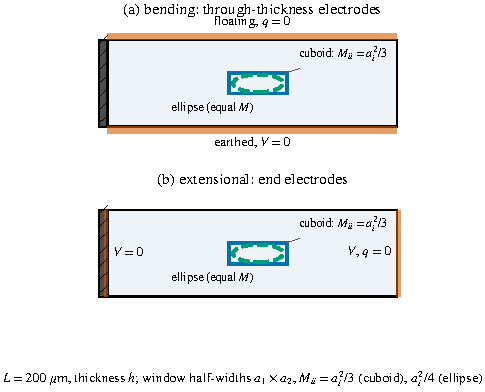
\includegraphics[width=0.72\textwidth]{P1_geometry.pdf}
\caption{The two electrode configurations and the averaging window.
(a) Bending family, poling $y$: electrodes cover the two large faces, the
lower earthed and the upper floating at $q=0$.  (b) Extensional family, poling
$x$: electrodes on the two shorter ends, one earthed and one floating.  In
both, the nonlocal window is either a rectangle of half-widths $a_1\times a_2$
(second moment $M_{ii}=a_i^2/3$) or an ellipse, and only the second-moment
tensor of the window enters the gradient energy; the two shapes drawn here are
the equal-$M$ pair, which is why they are not drawn to the same half-width.}
\label{fig:geometry}
\end{figure}

\subsection{Electrode conditions and coupling factors}
\label{sec:coupling}

Two electric boundary conditions are used throughout.  In the
\emph{short-circuit} configuration the electrode pair is grounded, the
internal potential dofs are condensed, and the mechanical problem has
stiffness $K_{sc}$.  In the \emph{open-circuit} configuration one electrode is
grounded, the other floats at a single potential $V$ with zero net charge,
which is again a condensation; the result is the rank-one update
\begin{equation}
  K_{oc} = K_{sc} + \frac{1}{\beta}\, d\,d^{\mathsf T},
  \label{eq:rankone}
\end{equation}
with $d$ the condensed coupling vector and $\beta$ the condensed dielectric
coefficient.  Two coupling measures follow, and the distinction between them
is the subject of Sec.~\ref{sec:couplingcare}.
\begin{enumerate}
\item the \emph{mode-based} factor of the $j$-th mode,
  $k_j^2=(\omega_{oc,j}^2-\omega_{sc,j}^2)/\omega_{oc,j}^2$;
\item the \emph{mode-free quasi-static} factor of the electrode pair,
  \begin{equation}
    x = \frac{d^{\mathsf T}K_{uu}^{-1}d}{\beta},\qquad
    k^2 = \frac{x}{1+x},
    \label{eq:kstatic}
  \end{equation}
  which involves no eigenvector at all.
\end{enumerate}
Equation~\eqref{eq:kstatic} is the measure used wherever a quantity has to be
compared across geometries, because it cannot select a different mode in a
different configuration.  Figure~\ref{fig:geometry} fixes the two electrode
arrangements that the index pairs in this paper refer to.

%% ===========================================================================
\section{Finite element implementation}
\label{sec:fem}
%% ===========================================================================

\subsection{Element matrices}

On the BFS rectangle the eight dofs of \eqref{eq:dofs} per node give, for an
element with nodal dof vector $\bm{u}^e$ of length $32$, the strain
$\varepsilon = B(\xi,\eta)\,\bm{u}^e$ and the strain gradient
$\eta=\partial_k\varepsilon = B_{,k}(\xi,\eta)\,\bm{u}^e$, both integrated by
$2\times2$ Gauss quadrature in the element frame.  The element contributions
are the elastic $K_e=\int B^{\mathsf T}CB$, the gradient
$K_{g,e}=\tfrac12\int M_{mn}B_{,m}^{\mathsf T}CB_{,n}$, the piezoelectric
coupling $B_{e}=\int B^{\mathsf T}e^{\mathsf T}\nabla N_\phi$ with a bilinear
potential interpolation $N_\phi$, the dielectric
$C_{\phi,e}=-\int\kappa\,\nabla N_\phi\cdot\nabla N_\phi$ and the mass matrix
from a consistent density interpolation.  The flexoelectric contribution is
assembled into $B_e$ as the additional potential--displacement coupling that
the $\mu_{kijl}\eta_{ijl}$ term of \eqref{eq:energy} produces; because it
involves $B_{,k}$, it is the only term for which the $C^1$ character of the
element is indispensable.

\subsection{Potential condensation}

The assembled system is indefinite in the saddle-point form
\begin{equation}
  \begin{bmatrix} K & B \\ B^{\mathsf T} & -C_\phi \end{bmatrix}
  \begin{bmatrix} \bm{u} \\ \bm{\phi}\end{bmatrix}
  = \begin{bmatrix} \bm{f} \\ \bm{q}\end{bmatrix},
  \label{eq:saddle}
\end{equation}
with $C_\phi$ projected to be positive.  Eliminating the potential dofs of the
electrode set reproduces \eqref{eq:rankone} exactly, and the returned pair
$(d,\beta)$ is what the modal and static solvers consume.  Two conventions are
enforced in the code because they are easy to get wrong: charge is read as
$q = d^{\mathsf T}\bm{u}/\beta$ rather than by pointwise integration of the
electric displacement, and eigenvectors are phase-normalised on a nodal
displacement dof (normalising on $\max|\phi|$ can select a derivative dof and
return a meaningless voltage -- an error observed at the $10^{-9}$\,V level).

\subsection{Time stepping and modal memory}
\label{sec:stepping}

With the L1 weights of \eqref{eq:l1} the time-discrete problem is
\begin{equation}
  \left(M + \Delta t^{\alpha}\Gamma(2-\alpha)\,K_{\rm mem}\right)\bm{a}^n
  = \bm{f}^n - K\bm{u}^n - K_{\rm mem}\sum_{k=1}^{n-1} b_{n-k}
    \left(\bm{u}^{k}-\bm{u}^{k-1}\right),
  \label{eq:step}
\end{equation}
solved by Cholesky factorisation of the constant left-hand matrix, with
$K_{\rm mem}\in\{K_{\rm eff},K_{uu}\}$ as the model choice
(Sec.~\ref{sec:memorystudy}).  For the modal variant the same convolution is
carried on the mass-normalised coordinates of the retained modes, so the cost
per step is $O(N_{\rm modes})$ rather than $O(N_{\rm dof})$; the truncation
error of that projection is measured in check~V6 and is reported in
Sec.~\ref{sec:verification} rather than assumed small.

\subsection{Damping ratio from the ring-down}
\label{sec:zeta}

The fractional model has no single damping ratio, so one is extracted from the
numerical ring-down.  The na\"ive metric -- the half-amplitude time -- was
found unusable on an oscillating response and was replaced by the logarithmic
decrement of successive peak amplitudes,
\begin{equation}
  \zeta_{\rm eff} = \frac{1}{2\pi}\,\ln\frac{A_k}{A_{k+1}},
  \label{eq:zeta}
\end{equation}
which is well defined for a lightly damped fractional system with
$\omega\tau=O(0.1-1)$.

%% ===========================================================================
%% sections 4-8 continue in the next block

%% ===========================================================================
\section{Verification}
\label{sec:verification}
%% ===========================================================================

The whole verification set is produced by a single command,
\texttt{python3 python/run\_all.py}, which runs the eight solver scripts and the
figure scripts and then grades fifty-one stated criteria, writing one
pass/fail table (\texttt{results/SUMMARY.md}) in about \SI{190}{\second}.  Nothing in this section is
graded inside the individual scripts: the criteria, their tolerances and their
values live in one place, so a reader can see exactly what was asserted.
Table~\ref{tab:verification} reproduces the table verbatim.

\begin{table}[t]
\centering
\small
\caption{Verification and validation table, generated by
\texttt{python/make\_paper\_table.py} from \texttt{results/summary.json} so
that it cannot drift from the run.  Values are the quantities named in the
criterion column; the tolerances were fixed before the runs.
\textbf{51/51 pass.}}
\label{tab:verification}
% generated by python/make_paper_table.py -- do not edit by hand
\begin{tabular}{@{}llll@{}}
\toprule
id & checked quantity & value & criterion \\
\midrule
V1a & patch test, relative energy error & $4.44\times10^{-16}$ & < $1\times10^{-12}$ \\
V1b & gradient energy at constant strain & $1.06\times10^{-12}$ & < $1\times10^{-9}$ \\
V1c & $K_g$(ellipsoid) vs FEM-1 closed form & $3.40\times10^{-16}$ & < $1\times10^{-12}$ \\
V1d & $K_g$(cuboid)/$K_g$(ellipsoid), equal half-width & 1.666667 & = 5/3 = 1.666667 \\
V1e & equal-$M$ cuboid vs ellipsoid & $0.00\times10^{0}$ & = 0 (< $1\times10^{-12}$) \\
V2 & tip displacement, length-scale sweep & 4.2339 \,\si{\micro\metre} & within 2 \% of 4.23 \,\si{\micro\metre} (paper) \\
V3 & observed order of convergence & 1.68 & > 1.5 \\
V4a & $C_\phi$ smallest eigenvalue & $2.27\times10^{-10}$ & < $1\times10^{-6}$ (no net charge in bending) \\
V4b & piezo extensional $k^2$ (poling $x$) & 0.3991 & > 0.35 \\
V5a & L1, $\alpha=1$, observed order & 0.99 & > 0.9 \\
V5b & L1 stencil error & 0.37 \% & < 2 \% \\
V5c & harmonic amplitude, $\alpha=1$ & $2.08\times10^{-9}$ & < $1\times10^{-6}$ \\
V5d & harmonic amplitude, $\alpha=0.5$ & 0.52 \% & < 1 \% \\
V6a & modal truncation, 24 modes & $3.19\times10^{-2}$ & < $5\times10^{-2}$ \\
V6b & truncation error monotone in $N_{\rm modes}$ & yes & monotone \\
V7 & equal-$M$ cuboid vs ellipsoid, max rel.\ diff & $0.00\times10^{0}$ & < $1\times10^{-12}$ \\
F1 & flexo patch test, $\mu=0$ & $0.00\times10^{0}$ V & = 0 \\
F2 & flexo patch test, $\mu\neq0$ & 1.0000000000 & = 1 ($1\times10^{-10}$) \\
F3 & linearity of the flexo response in $\mu$ & 2.0000000000 & = 2 \\
F4 & bending $k^2$ with $\mu=10^{-6}$\,\si{\coulomb\per\metre} & $1.25\times10^{-4}$ & > $1\times10^{-5}$ \\
M1 & $\kappa_{11}/\kappa_{33}$ of the material record & 39.3 & > 30 (real crystal, was 1.2) \\
S1a & $\zeta_{\rm eff}(K_{\rm eff},\alpha{=}1)$ vs $\omega\tau/2$ & 0.15023 vs 0.15000 & within 2 \% \\
S1b & $\zeta(K_{uu})/\zeta(K_{\rm eff})$, $\alpha=1$ & 0.449 & in (0, 1) -- the choice matters \\
S2 & KV/Zener modulus, $\omega\tau=1$, $\alpha=1$ & 1.345 & > 1.3 (KV unbounded) \\
C1 & FEM $k^2$ (free plate) vs 2-D closed form $e^{\rm T}C^{-1}e/\kappa$ & 0.56079 vs 0.56079 & rel. diff < $1\times10^{-3}$ \\
C2 & 2-D model vs 3-D free bar (plane-stress reduction) & 2.83 \% & < 5 \% (doc\,\si{\micro\metre}ented modelling gap) \\
C3 & FEM $k^2$, clamped, $96\times4$ vs $48\times4$ & 0.55992 vs 0.55957 & rel. diff < $1\times10^{-3}$ \\
C4 & FEM $k^2$, clamped, $24\times2$ vs $48\times4$ & 0.13 \% & < 0.5 \% (coarse mesh) \\
K1 & lowest MAC of mode 1, $h=10\to1$\,\si{\micro\metre} & 0.99919 & > 0.999 \\
K2 & worst MAC off-diagonal / $f_2/f_1$ & $2.3\times10^{-6}$, f2/f1 >= 6.21 & off-diag < $1\times10^{-5}$, ratio > 6 \\
D1 & closed form e'C\^{}-1 e/kappa vs FEM coupling (free plate) & 0.56079 vs 0.56079 & rel. diff < $1\times10^{-3}$ \\
D2 & the superseded series is exactly k\^{}2/(1+k\^{}2) of the new one & $3.5\times10^{-6}$ & < $1\times10^{-5}$ (same formula applied twice) \\
I1 & clamped-free f1, FEM 48x4 vs Euler-Bernoulli closed form & 144.6 vs 143.8 \,\si{\kilo\hertz} & |err| < 1 \% (+0.54 \%) \\
I2 & clamped-clamped f1, FEM 48x4 vs Euler-Bernoulli closed form & 919.2 vs 915.0 \,\si{\kilo\hertz} & |err| < 1 \% (+0.46 \%) \\
I3 & clamped-free f1 at 128x4 vs Euler-Bernoulli (mesh refinement) & 144.08 \,\si{\kilo\hertz} & |err| < 0.5 \% (+0.20 \%) \\
I4 & zeta from Newton pole vs polynomial roots (10 alpha, 2 omega*tau) & $1.4\times10^{-10}$ & < $1\times10^{-8}$ \\
I5 & zeta at alpha = 1 vs omega*tau/2 (both omega*tau) & $0.0\times10^{0}$ & < $1\times10^{-9}$ \\
I6 & flexo x, uniform curvature: FEM energy triple vs 3 mu\^{}2/(C11 h\^{}2 kappa33) & $3.570415\times10^{-4}$ vs $3.570415\times10^{-4}$ & rel. diff < $1\times10^{-8}$ (worst $1.8\times10^{-10}$) \\
I7 & flexo Voc, uniform curvature: FEM vs mu*kappa*h/kappa33 & $1.7\times10^{-13}$ & < $1\times10^{-10}$ \\
A2 & every number in the abstract has an independent-check verdict & 10 hua / 7 nahi hua / 4 inputs, 20 tokens & 0 uncovered, 0 stale \\
G1 & piezoelectric share of the bending device (poling y, long faces) at every thickness & $5.7\times10^{-7}$ & < $1\times10^{-5}$ (electrically silent bending mode) \\
G2 & flexo growth with and without the piezoelectric terms & 23.9 vs 31.1 & reported 24 (2 s.f.) uses the real crystal; 31 with e = 0, both graded at 1 \% \\
I9 & the same bending field, four poling/electrode pairings: only the long faces collect it, and each pairing with its own permittivity & poled y $3.570\times10^{-4}$ vs $3.570\times10^{-4}$; poled x $1.613\times10^{-5}$ vs $1.613\times10^{-5}$; short-face pairs $7.5\times10^{-14}$ V & rel. diff < $1\times10^{-6}$, short-face charge < $1\times10^{-12}$ \\
I8 & window second-moment factors 1/3, 1/4, 1/5 by quadrature & $3.3\times10^{-6}$ & < $1\times10^{-5}$ \\
U1 & h = 1 um flexo k\^{}2 over four equivalent solver paths and 3 numeric stacks & spread 0.107 \%, k\^{}2 $4.1705\times10^{-3}$..$4.1781\times10^{-3}$ & < 0.5 \% (quoted to 2 s.f.) \\
U2 & the same spread at h = 10 um & $1.12\times10^{-5}$ \% & < $1\times10^{-3}$ \% \\
U3 & truncating the secular sum to 12 modes is not an alternative & 85 \% off & > 50 \% (hence the s\,\si{\micro\metre} runs over all modes) \\
N2 & the list of unverified numbers cites only numbers still in the manuscript & 31 entries, 0 stale & 0 stale \\
A1 & application table: extensional plane stress is the strongest coupling of the four & 0.4580 & = 0.4580, largest, > 0.4 \\
T1 & piezo $k^2$ (mode-free), max/min over $h$ & 1.0009 & < 1.005 (thickness independent) \\
T2 & piezo $k^2$, $24\times2$ vs $48\times4$ & $5.7\times10^{-4}$ & < $1\times10^{-3}$ \\
T3 & flexo $k^2$ vs $h$ & $1.74\times10^{-4}$ -> $4.17\times10^{-3}$ & strictly increasing as h falls \\
T4 & flexo $k^2$, $48\times4$ vs $96\times4$ witness & $3.5\times10^{-3}$ & < 0.02 \\
T5 & flexo $k^2$ at $\mu=0$, residual / value & $6\times10^{-7}$ & < $1\times10^{-5}$ \\
P1 & paper figure set, vector files written & 10 PDF & = 10 (P1-P10) \\
P2 & orientation sweep, rows / $k^2$ range & 168 rows, 0.3786-0.4677 & 168 rows (144 cuboid + 24 ellipse), k\^{}2 in (0.35, 0.50) \\
N1 & manuscript numbers vs the JSON they came from & 52/52 & all agree \\
\bottomrule
\end{tabular}

\end{table}

\subsection{Independent routes to the same numbers}
\label{sec:independent}

Every value in Table~\ref{tab:verification} comes out of the same assembly, so
a mistake shared by both sides of a comparison would survive it.  Eight of the
headline numbers are therefore re-derived along routes that never touch the
assembled matrices -- closed-form beam theory, the roots of a polynomial, and
the three scalars (charge, bending energy, capacitance) that fix a
one-degree-of-freedom coupling -- and a ninth criterion, I9, fixes which
modulus and which permittivity belong to which of the two poling
configurations of Table~\ref{tab:axes}.  Table~\ref{tab:independent} collects them; the
script is \texttt{python/run\_independent\_checks.py} and the criteria are
I1--I9.

\begin{table}[t]
\centering
\small
\caption{The headline numbers against independent routes.  (a) Fundamental
frequency of an elastic strip with $e=\mu=0$ and the gradient term switched
off, against the Euler--Bernoulli and Timoshenko closed forms evaluated with
the plane-stress \emph{beam} modulus $E_b=1/(\bm C_p^{-1})_{xx}$.  (b) Damping
ratio of the fractional Kelvin--Voigt element: the Newton pole of
\texttt{complex\_frequency} against the roots of the same equation rewritten
as a polynomial.  (c) Flexoelectric coupling in the uniform-curvature limit:
the finite element energy triple $\beta V^2/(u^{\mathsf T}Ku)$ against
$x=3\mu^2/(C^p_{xx}h^2\kappa_{yy})$ for the plate poled along $y$; panel
(e) puts all four poling/electrode pairings of the same field side by side.
(d) The second-moment factors of the
three window shapes, integrated over the shapes rather than read off the
formula in the code.  Generated by \texttt{run\_independent\_checks.py} from
\texttt{results/independent\_checks.json}.}
\label{tab:independent}
% generated by python/run_independent_checks.py -- do not edit
\begin{tabular}{@{}lrrrr@{}}
\toprule
boundary & Euler--Bernoulli & Timoshenko & FEM & error\\
& [kHz] & [kHz] & [kHz] & vs EB [\%]\\
\midrule
\multicolumn{5}{@{}l}{\emph{(a) elastic strip, $e=\mu=0$, no gradient term, $48\times4$ mesh}}\\
clamped\textendash free & 143.8 & 143.7 & 144.6 & +0.54\\
clamped\textendash clamped & 915.0 & 909.7 & 919.2 & +0.46\\
\midrule
\multicolumn{5}{@{}l}{\emph{(b) damping ratio: Newton pole of the pole equation against its polynomial roots}}\\
$\omega\tau$ & $\alpha$ & \multicolumn{2}{c}{$\zeta$: Newton / polynomial} & $\omega\tau/2$\\
\midrule
0.3 & 1 & 0.150000 & 0.150000 & 0.150000\\
0.3 & 0.9 & 0.166079 & 0.166079 & 0.150000\\
0.3 & 0.7 & 0.179384 & 0.179384 & 0.150000\\
0.3 & 0.5 & 0.158580 & 0.158580 & 0.150000\\
0.3 & 0.3 & 0.107711 & 0.107711 & 0.150000\\
1 & 1 & 0.500000 & 0.500000 & 0.500000\\
1 & 0.9 & 0.480460 & 0.480460 & 0.500000\\
1 & 0.7 & 0.370619 & 0.370619 & 0.500000\\
1 & 0.5 & 0.245360 & 0.245360 & 0.500000\\
1 & 0.3 & 0.134530 & 0.134530 & 0.500000\\
\midrule
\multicolumn{5}{@{}l}{\emph{(c) flexoelectric coupling, uniform curvature: $x=3\mu^2/(C^p_{11}h^2\kappa_{33})$ against the finite element energy triple}}\\
mesh & \multicolumn{2}{c}{$V_{oc}$ [V]: FEM / closed form} & $x$: FEM & $x$: closed form\\
\midrule
8$\times$2 & \multicolumn{2}{c}{2.016802e-02 / 2.016802e-02} & 3.570415e-04 & 3.570415e-04\\
24$\times$4 & \multicolumn{2}{c}{2.016802e-02 / 2.016802e-02} & 3.570415e-04 & 3.570415e-04\\
48$\times$8 & \multicolumn{2}{c}{2.016802e-02 / 2.016802e-02} & 3.570415e-04 & 3.570415e-04\\
96$\times$4 & \multicolumn{2}{c}{2.016802e-02 / 2.016802e-02} & 3.570415e-04 & 3.570415e-04\\
\midrule
\multicolumn{5}{@{}l}{\emph{(d) second moments of the window shapes: quadrature against the printed factor}}\\
shape & \multicolumn{2}{c}{$M_{11}$} & \multicolumn{2}{c}{$M_{22}$}\\
\midrule
cuboid & \multicolumn{2}{c}{0.3333333333 ($a_1^2/3$)} & \multicolumn{2}{c}{0.1200000000 ($a_2^2/3$)}\\
ellipse (2-D) & \multicolumn{2}{c}{0.2499991667 ($a_1^2/4$)} & \multicolumn{2}{c}{0.0900000000 ($a_2^2/4$)}\\
ellipsoid (3-D) & \multicolumn{2}{c}{0.2000000000 ($a_1^2/5$)} & \multicolumn{2}{c}{0.0720000000 ($a_2^2/5$)}\\
\bottomrule
\end{tabular}

\end{table}

\paragraph{The elastic strip.}  With the piezoelectric and flexoelectric
couplings removed the plate is a \SI{200}{\micro\metre} by
\SI{10}{\micro\metre} elastic strip, and its fundamental is predicted to
$0.5\,\%$ by Euler--Bernoulli theory (I1, I2); refining the mesh in the axial
direction brings the clamped--free value from \SI{144.6}{\kilo\hertz} at
$48\times4$ to \SI{144.08}{\kilo\hertz} at $128\times4$ against
\SI{143.8}{\kilo\hertz} (I3).  The check also settles a modelling question that
the finite element model itself cannot: the modulus that appears is the beam
modulus $E_b=\SI{7.63e10}{\pascal}$, not the plane-stress modulus
$C^p_{11}=\SI{9.55e10}{\pascal}$ that a wide plate of the same orientation
would use; both belong to the plate poled along $x$, the orientation used
throughout except in the flexoelectric check below (Table~\ref{tab:axes}).  The two differ
by $25\,\%$, so the $0.5\,\%$ agreement is not a coincidence of the tolerance
chosen.  The clamped--clamped case follows the same pattern: \SI{919.2}{\kilo\hertz} against \SI{915.0}{\kilo\hertz}.  Timoshenko's correction moves the closed form down by $1\,\%$ (Table~\ref{tab:independent}a), and the $C^1$ element sits at the Kirchhoff limit rather than the Timoshenko one, as an element with no
transverse shear strain must.

\paragraph{The fractional pole.}  For a rational order $\alpha=p/q$ the pole
equation $s^2+\omega_0^2(1+(\tau s)^\alpha)=0$ becomes a polynomial of degree
$2q$ in $w=s^{1/q}$; each of its roots is checked against the original
equation, and the one on the principal branch is kept.  Over five orders
$\alpha\in\{1,0.9,0.7,0.5,0.3\}$ and two decades of $\omega\tau$ the two routes
agree to $1.4\times10^{-10}$ (I4), and at $\alpha=1$ both return $\omega\tau/2$
exactly (I5).  The table is worth reading for its shape as well as its
agreement: at $\omega\tau=0.3$ the damping ratio is \emph{not} monotone in
$\alpha$ -- it rises from $0.150$ at $\alpha=1$ to $0.179$ at $\alpha=0.7$ and
then falls to $0.108$ at $\alpha=0.3$.  A fractional element is therefore not a
small perturbation of the integer one even when $\omega\tau\ll1$, which is the
reason the order has to be carried explicitly.

\paragraph{The flexoelectric coupling.}  The constant-strain patch test
(check~F2) fixes the open-circuit voltage of the flexoelectric model, but says
nothing about the stiffness or the capacitance that the coupling factor
divides by.  Imposing the pure-bending field
$u=\kappa xy$, $v=-\kappa x^2/2$ -- a uniform strain gradient, and a
\emph{quadratic} displacement field rather than a constant one -- gives one
degree of freedom for which charge, energy and capacitance are all known in
closed form, and the finite element value
$x=\beta V^2/(u^{\mathsf T}Ku)$ reproduces
\begin{equation}
  x=\frac{3\mu^2}{C^p_{xx}h^2\kappa_{yy}}=3.570415\times10^{-4}
\end{equation}
to $2\times10^{-10}$ on four different meshes (I6, I7).

Three details make this more than a restatement of the patch test.  First, the
neutral axis of the imposed field lies on the edge $y=0$, so the bending
energy carries $\int_0^hy^2\,dy=h^3/3$ and not the mid-plane $h^3/12$ -- a
factor of four that a formula quoted for a beam about its centroid would get
wrong.  Second, the field has $\varepsilon_{yy}=0$ exactly, so the modulus
that enters is the constrained $C^p_{xx}$ and not the beam modulus.  Third,
and this is the part the notation has to carry: the plate in this check is
poled along $y$, across the thickness, because the flexoelectric polarization
of the field, $\bm D=\mu\kappa\hat{\bm y}$, is normal to the long faces and
would be collected by no electrode at all on the short ones.  For that
orientation $C^p_{xx}=\SI{1.6946e11}{\pascal}$ and
$\kappa_{yy}=\kappa_{33}$,
whereas the plate of Step~3 is poled along $x$ and its $C^p_{xx}$ is the
$\SI{9.55e10}{\pascal}$ of Table~\ref{tab:closedform}.  The two are the same
symbol in two orientations, not two estimates of one number;
Table~\ref{tab:axes} sets the axes, the indices and the two tensors side by
side, and the beam modulus of the poling-$y$ plate is
\SI{1.3544e11}{\pascal}.

\paragraph{The modulus and the permittivity must come from one configuration.}
The arithmetic invites a slip that is worth closing explicitly, because the
right answer is not obvious from the formula alone.  Taking the modulus of
Step~3, $\SI{9.55e10}{\pascal}$, together with the poling-$y$ permittivity
$\kappa_{33}$ gives $x=6.34\times10^{-4}$, $77\,\%$ away from the finite
element value -- and no poling/electrode pairing of this geometry produces
that number.  With the poling along $x$ the plate is electroded on its short
faces, where $\bm D=\mu\kappa\hat{\bm y}$ is parallel to the electrode and
the collected charge is zero to round-off; putting the electrodes on the long
faces of a poling-$x$ plate instead changes the permittivity to
$\kappa_{11}=39\kappa_{33}$ and gives $x=1.61\times10^{-5}$, an order of
magnitude smaller than either.  Panel~(e) of Table~\ref{tab:independent} is
the four configurations, and only the first reproduces the finite element
solution (I9).

\paragraph{The window shapes.}  The second-moment factors
$a_i^2/3$, $a_i^2/4$ and $a_i^2/5$ are asserted throughout
Sec.~\ref{sec:window}; here they are obtained by integrating $r_i^2$ over each
shape and dividing by its measure (I8).  The agreement, $3.3\times10^{-6}$ --
the residual is the trapezoid rule in the polar angle -- confirms that the
factors are the geometric second moments the argument claims and not fitted
constants.

\subsection{Material record and the plane-stress/plane-strain choice}
\label{sec:material}

The material is tetragonal BaTiO$_3$ at room temperature, with the elastic,
piezoelectric and dielectric constants of Zgonik~et~al.~\cite{zgonik}:
$C_{11}=2.22\times10^{11}$, $C_{12}=1.08\times10^{11}$,
$C_{13}=1.11\times10^{11}$, $C_{33}=1.51\times10^{11}$,
$C_{44}=6.10\times10^{10}$\,Pa; $e_{15}=34.2$, $e_{31}=-0.7$,
$e_{33}=6.7$\,\si{\coulomb\per\square\metre};
$\kappa_{11}/\kappa_0=2200$, $\kappa_{33}/\kappa_0=56$.  The dielectric
anisotropy ratio is therefore $39.3$ (check~M1); a record with an isotropic
or near-isotropic dielectric tensor would give $\simeq1.2$ and is rejected by
that check.  The mass density $\rho=\SI{6020}{\kilo\gram\per\cubic\metre}$
is \emph{unverified} against a primary source and is flagged as such: it
affects every frequency in this paper by a common factor and no conclusion
here depends on its value.

Two electrical configurations of this one geometry are used below, and they
differ in the poling axis; since the crystal is anisotropic, they also differ
in which entry of the plane-stress tensor multiplies $\varepsilon_{xx}$.
Table~\ref{tab:axes} fixes the axes, the Voigt indices and the two tensors
once, so that every later formula can be read against it.  The extensional
coupling is computed with the poling along $x$ (electrodes on the short faces,
gap $L$); the flexoelectric bending check and the thickness sweep of
Sec.~\ref{sec:thickness} are poled along $y$ (electrodes on the long faces,
gap $h$), because the strain gradient of a bending mode is carried across the
thickness and only that pairing collects it.

\begin{table}[t]
\centering
\small
\caption{Which axis, which Voigt index, which modulus.  (a) The axes of the
model: Voigt indices are $1=x$, $2=y$, $3=z$ throughout, and $z$ is a basal
direction of the $4mm$ crystal in both orientations.  (b) The two
configurations used in the paper.  They share the geometry and the material
record but not the poling axis, and a modulus may only be paired with the
permittivity of its own configuration -- the pairing of the poling-$x$
modulus with the poling-$y$ permittivity is examined, and excluded, in
Sec.~\ref{sec:independent}.  Generated by
\texttt{run\_independent\_checks.py} from
\texttt{results/independent\_checks.json}.}
\label{tab:axes}
% generated by python/run_independent_checks.py -- do not edit
\begin{tabular}{@{}llll@{}}
\toprule
\multicolumn{4}{@{}l}{\emph{(a) the model axes, Voigt indices $1=x$, $2=y$, $3=z$}}\\
axis & role & extent & what it carries\\
\midrule
$x$ & length & \SI{200}{\micro\metre} & bending: $\varepsilon_{xx}=\kappa y$; the piezoelectric load direction\\
$y$ & thickness & \SI{10}{\micro\metre} & strain gradient $\partial\varepsilon_{xx}/\partial y=\kappa$; the flexoelectric gap\\
$z$ & out of plane & -- & neutral axis of the bending (curvature about $z$), free surface\\
\midrule
\multicolumn{4}{@{}l}{\emph{(b) the two configurations; they differ in the poling axis, and therefore in which entry of $\bm C_p$ multiplies $\varepsilon_{xx}$}}\\
& & piezo $k^2$ (\ref{sec:closedform}) & flexo check (\ref{sec:independent})\\
\midrule
poling axis & & $x$ & $y$\\
electrodes & & $x=0$, $x=L$ (short faces) & $y=0$, $y=h$ (long faces)\\
gap & & $L=$\SI{200}{\micro\metre} & $h=$\SI{10}{\micro\metre}\\
permittivity across the gap & & $\kappa_{xx}=\kappa_{33}=$\SI{4.9583e-10}{\farad\per\metre} & $\kappa_{yy}=\kappa_{33}=$\SI{4.9583e-10}{\farad\per\metre}\\
$C^p_{xx}$ & multiplies $\varepsilon_{xx}$ & \SI{9.5500e10}{\pascal} & \SI{1.6946e11}{\pascal}\\
$C^p_{yy}$ & & \SI{1.6946e11}{\pascal} & \SI{9.5500e10}{\pascal}\\
$E_b=1/(\bm C_p^{-1})_{xx}$ & beam modulus & \SI{7.6327e10}{\pascal} & \SI{1.3544e11}{\pascal}\\
coupling & & $\bm e_p^{\mathsf T}\bm C_p^{-1}\bm e_p/\kappa_{xx}$ & $3\mu^2/(C^p_{xx}h^2\kappa_{yy})$\\
\bottomrule
\end{tabular}

\end{table}

Because the plate is discretised as a 2-D continuum, the constitutive
reduction is part of the model.  Table~\ref{tab:kinematics} compares the two
choices on the \SI{200}{\micro\metre}$\times$\SI{10}{\micro\metre} plate with a
$24\times2$ mesh.  The plane-stress reduction is adopted throughout, on the
grounds that a free plate is thin out of plane and nothing constrains it
there; the table is included because the difference is large enough to matter
for the extensional case and because the earlier papers in this
series~\cite{fem4,fem5} used plane strain.

\begin{table}[t]
\centering
\small
\caption{Plane strain versus plane stress for the
\SI{200}{\micro\metre}$\times$\SI{10}{\micro\metre} plate, $24\times2$ mesh.
$f_1$ is the fundamental; $f$, $k^2$ and $V_0$ belong to the mode that carries
the largest coupling in that configuration (its index in the sixth column),
because that is the mode a harvester would be driven at.  Mixing an $f_1$
from the fundamental with a $k^2$ from a higher mode is a common way of
producing a table that no single eigenvector supports, and it is avoided here
by keeping both frequencies.  $V_0$ is the open-circuit voltage when the
largest nodal displacement in the mode is \SI{10}{\nano\metre}.
Generated by \texttt{python/run\_application\_table.py}.}
\label{tab:kinematics}
\par\smallskip
{\scriptsize
\begin{tabular}{@{}llcccccc@{}}
\toprule
& & & \multicolumn{2}{c}{$f$ (kHz)} & & & \\
\cmidrule(lr){4-5}
poling & mode & kinematics & $f_1$ & $f_{\rm mode}$ & index & $k^2$ & $V_0$ (V) \\
\midrule
$y$ (bending)     & $y$-coupled & plane strain & 220.46 & 6721.8 & 4 & 0.1749 & 3.48 \\
$y$ (bending)     & $y$-coupled & plane stress & 208.73 & 6361.0 & 4 & 0.1141 & 2.41 \\
$x$ (extensional) & $x$-coupled & plane strain & 165.57 & 7161.0 & 5 & 0.4024 & 141.45 \\
$x$ (extensional) & $x$-coupled & plane stress & 147.73 & 6725.8 & 5 & 0.4580 & 138.99 \\
\bottomrule
\end{tabular}}
\end{table}

\subsection{Patch tests and exact identities}
\label{sec:patch}

The first group of checks is exact, and each one is a statement that can be
verified by hand.
\begin{itemize}
\item A constant-strain field must produce exactly the classical strain
  energy: $4.4\times10^{-16}$ relative error (V1a), and a constant-strain
  field must produce \emph{no} gradient energy, $1.06\times10^{-12}$ (V1b).
  The second is the one that detects a wrong derivative operator in
  \eqref{eq:Kg}.
\item The strain-gradient coefficient of an ellipsoidal window must reduce to
  the closed form used in the earlier $C^1$ plate work~\cite{fem1}; the
  discrepancy is $3.4\times10^{-16}$ (V1c).
\item The cuboid-to-ellipsoid ratio at equal half-width must be
  $M^{\rm cub}_{ii}/M^{\rm ell}_{ii}=(1/3)/(1/5)=5/3$, returned as
  $1.666667$ (V1d).
\item Two windows with the \emph{same} $M$ must produce identical solutions,
  to the level of round-off: $0.00$ (V1e, V7).  This is the practical content
  of \eqref{eq:Mdef} and it is the reason the window shape is not a modelling
  choice once its second moment is fixed.
\end{itemize}

The flexoelectric group is the same idea applied to the coupling term.  With
$\mu=0$ the flexoelectric contribution must vanish exactly (\SI{0}{\volt},
F1).  With $\mu\neq0$ a prescribed uniform curvature must produce the
potential predicted by the patch solution, and the ratio to the analytical
value $\mu\kappa h/\kappa_{33}$ is $1.0000000000$ (F2), independent of the
mesh ($4\times1$, $8\times2$, $24\times2$) and linear in $\mu$
($2.0000000000$ for a doubling of $\mu$, F3).  A closed form for the
cantilevered flexoelectric voltage that had been proposed earlier,
$\mu h\theta_{\rm tip}/(\kappa_{33}L)$, was found to be wrong in the course of
this work and is \emph{not} used; the patch solution above replaces it.

\subsection{Benchmarks, convergence and the time discretisation}

Check V2 reproduces the tip displacement of the earlier $C^1$ plate
benchmark~\cite{fem1} at a length-scale ratio $\ell/L=0.2$:
\SI{4.2339}{\micro\metre} against the published \SI{4.23}{\micro\metre}, with
the classical value \SI{4.5}{\micro\metre} recovered as $\ell/L\to0$
($0.9974$ at $\ell/L=0.02$).  The observed order of convergence of the BFS
discretisation on that problem is $1.68$ on the sequence $5\times1\to
40\times8$ (V3), which is the order expected for an element whose error is
dominated by the cross-derivative continuity.

For the fractional part, the L1 scheme is checked three ways: the observed
order at $\alpha=1$ is $0.99$ (V5a); the delivered stencil itself is compared
against an exact reference and reproduces it to $0.37\,\%$ (V5b); and the
steady-state amplitude of a harmonically forced fractional oscillator is
compared with the closed-form solution of \eqref{eq:kvfreq}, giving
$2.08\times10^{-9}$ absolute at $\alpha=1$ and $0.52\,\%$ relative at
$\alpha=0.5$ (V5c, V5d).  The modal truncation study (V6) is reported rather
than hidden: with 24 retained modes the tip displacement is $3.19\times10^{-2}$
short of the direct solution, and the error decreases monotonically with the
number of modes, which is the property the modal memory scheme needs.

\subsection{The coupling factor from the material constants}
\label{sec:closedform}

Before the coupling factor is used anywhere, it is worth obtaining it without
the finite element code at all.  The quasi-static factor of an electrode pair
is
\begin{equation}
  x=\frac{d^{\mathsf T}K_{uu}^{-1}d}{\beta},\qquad k^2=\frac{x}{1+x},
  \label{eq:kx}
\end{equation}
with $K_{uu}$ the \emph{short-circuit} stiffness; for a homogeneous body whose
strain is free, the same $x$ follows from the constitutive tensors, because the
mechanical energy released by the polarisation is $\tfrac12\bm e^{\mathsf T}
\bm C^{-1}\bm e\,E^2$ per unit volume against $\tfrac12\kappa E^2$ of
electrical energy:
\begin{equation}
  x=\frac{\bm e^{\mathsf T}\bm C^{-1}\bm e}{\kappa},\qquad k^2=\frac{x}{1+x}.
  \label{eq:kclosed}
\end{equation}
Nothing in \eqref{eq:kclosed} knows about the mesh, the element, the potential
condensation or the floating-electrode update, so the comparison of the two is
a check of the whole piezoelectric path.

\paragraph{Step 1: the record.}  Poling along $x$ makes the polar axis the
$3$-axis, so the 3-D stiffness in the $(x,y,z)$ frame is
\begin{equation}
  \bm C_3=\begin{pmatrix}C_{33}&C_{13}&C_{13}\\ C_{13}&C_{11}&C_{12}\\
  C_{13}&C_{12}&C_{11}\end{pmatrix}
  =\begin{pmatrix}15.10&11.10&11.10\\ 11.10&22.20&10.80\\
  11.10&10.80&22.20\end{pmatrix}\times10^{10}\ \mathrm{Pa},
\end{equation}
and the piezoelectric row that couples to the field along $x$ is
$\bm e_3=(e_{33},e_{31},e_{31})=(6.7,-0.7,-0.7)$\,\si{\coulomb\per\metre\squared}
with $\kappa_{33}=56\varepsilon_0=\SI{4.9583e-10}{\farad\per\metre}$.

\paragraph{Step 2: the three-dimensional free bar.}
With every normal strain free, $\bm s_3=\bm C_3^{-1}$ and
\begin{equation}
  x_{3D}=\frac{\bm e_3^{\mathsf T}\bm s_3\bm e_3}{\kappa_{33}}
  =\frac{6.7667\times10^{-10}}{4.9583\times10^{-10}}=1.3647,
  \qquad k^2_{3D}=\frac{1.3647}{2.3647}=0.5771 .
\end{equation}
The blocked textbook value is $k_{33}^2=e_{33}^2/(C_{33}\kappa_{33})=0.5996$,
whose free counterpart $k^2=x/(1+x)$ with $x=k_{33}^2$ is $0.3748$: the three
numbers $0.5771$, $0.5996$ and $0.3748$ differ only in how much the body is
allowed to relax, and a table that quotes one of them without saying which is
a common source of disagreement.

\paragraph{Step 3: the plane-stress reduction.}  The model is plane stress,
$\sigma_{zz}=0$, so the out-of-plane normal is condensed.  The plate here is
poled along $x$, the length, so $x$ is the polar axis and the electrodes are
the end faces; the Voigt indices used from this point on are $1=x$, $2=y$,
$3=z$, and $C_{33}^{(zz)}=C_{11}$ is the modulus of the out-of-plane basal
direction (Table~\ref{tab:axes}).  The condensation is
\begin{equation}
  \bm C_p=\bm C_{2d}-\frac{\bm c_3\bm c_3^{\mathsf T}}{C_{33}^{(zz)}},
  \qquad \bm c_3=(11.10,\,10.80)\times10^{10}\ \mathrm{Pa},
\end{equation}
\begin{equation}
  \bm C_p=\begin{pmatrix}9.5500&5.7000\\ 5.7000&16.9459\end{pmatrix}\times10^{10}\
  \mathrm{Pa},\qquad C_{44}=6.10\times10^{10}\ \mathrm{Pa}.
\end{equation}
The reduction carries its own check: the plane-stress compliance must be the
corresponding block of the 3-D compliance, and here
$\max|\bm C_p^{-1}-(\bm s_3)_{2\times2}|=3\times10^{-27}$\,\si{\per\pascal},
i.e.\ exact.  The piezoelectric and dielectric tensors are \emph{not} reduced:
with $\sigma_{zz}=0$ and $D_z=0$ the eliminated out-of-plane strain re-enters
only through the $e_{31}$ terms that the in-plane block already contains, so
$\bm e_p=\bm e_{2d}$ and $\kappa_{\rm eff}=\kappa_{xx}=\kappa_{33}$.

\paragraph{Step 4: the two-dimensional closed form.}  With
$\bm e_p=(6.7,-0.7,0)$ and $\bm C_p^{-1}$ as above,
\begin{equation}
  \bm e_p^{\mathsf T}\bm C_p^{-1}\bm e_p=6.3308\times10^{-10}\
  \frac{\mathrm{C}^2}{\mathrm{N\,m^2}},\quad
  \kappa_{xx}=4.9583\times10^{-10}\ \frac{\mathrm{F}}{\mathrm{m}},
\end{equation}
\begin{equation}
  x=\frac{6.3308}{4.9583}=1.2768,\qquad
  k^2=\frac{1.2768}{2.2768}=0.5608 .
\end{equation}
The arithmetic can be repeated by hand from
$\det\bm C_p=1.2934\times10^{22}\,\mathrm{Pa}^2$ and the three numbers above;
no step needs the finite element code.

\paragraph{Step 5: the finite element model against it.}
Table~\ref{tab:closedform} puts the two side by side.  The unconstrained plate
reproduces the closed form to the fifth decimal ($0.56079$ against $0.56079$),
which is the check that the $e$ tensor, the plane-stress reduction, the
condensation of the internal potential dofs and the rank-one electrode update
are all consistent with each other and with \eqref{eq:kclosed}.  Clamping one
edge lowers the coupling by $0.2\,\%$ and refining the mesh recovers it
monotonically ($0.55884\to0.55957\to0.55992$), so the clamping is a physical
boundary effect and the remaining gap is discretisation.  The plane-strain
model gives $0.5132$ against a finite element value of $0.5115$; the
$2.8\,\%$ gap between the 2-D plane-stress value and the 3-D free bar is the
$\sigma_{zz}=0$ assumption itself, not the discretisation, and it is reported
separately for that reason.

\begin{table}[t]
\centering
\small
\caption{The extensional coupling factor of the
\SI{200}{\micro\metre}$\times$\SI{10}{\micro\metre} BaTiO$_3$ plate: constitutive
closed forms \eqref{eq:kclosed} against the finite element model of the same
plate.  $x$ is the reduced coupling of \eqref{eq:kx}.  The finite element
values contain no material input beyond the record of Step 1; the closed form
contains no geometry.  Generated by
\texttt{python/derive\_k2\_closed\_form.py}.}
\label{tab:closedform}
% table generated from the archived results
\begin{tabular}{@{}lcc@{}}
\toprule
& $x$ & $k^2$ \\
\midrule
3-D free bar & 1.3647 & 0.5771 \\
3-D uniaxial ($k_{33}^2$) & 0.5996 & 0.3748 \\
2-D plane stress, from the record & 1.3542 & \textbf{0.5752} \\
\midrule
FEM, plane stress, free, $48\times4$ & 1.3542 & \textbf{0.57523} \\
FEM, plane stress, clamped, $24\times2$ & 1.3441 & 0.57339 \\
FEM, plane stress, clamped, $48\times4$ & 1.3480 & 0.57410 \\
FEM, plane stress, clamped, $96\times4$ & 1.3498 & 0.57444 \\
\midrule
2-D plane strain, from the record & 1.0541 & 0.5132 \\
FEM, plane strain, clamped, $48 \times 4$ & 1.0471 & 0.5115 \\
\bottomrule
\end{tabular}

\end{table}

\subsection{A cautionary note on coupling factors}
\label{sec:couplingcare}

Three of the measurements in this paper are easy to get wrong -- two because
they are differences of nearly equal numbers, one because the same coupling map
was applied twice -- and all three produced smooth, plausible, wrong numbers
before they were reformulated.  They are reported here because a reader who
re-implements the method will meet them.

\paragraph{Mode selection.}  If the coupling factor of a plate is read as the
largest $k^2$ among the first fourteen modes, then thinning the plate moves
the argmax from mode 5 to 6 to 8 to 10, and the resulting curve is
non-monotone ($0.4580$, $0.4520$, $0.3128$, $0.3621$ for
$h=10,5,2,1$\,\si{\micro\metre}) although nothing physical has changed: the
coupling of the plate is a property of its cross-section, not of which mode
happens to be largest at a given thickness.  The remedy is to use a measure
that contains no eigenvector, \eqref{eq:kstatic}.

\begin{figure}[t]
\centering
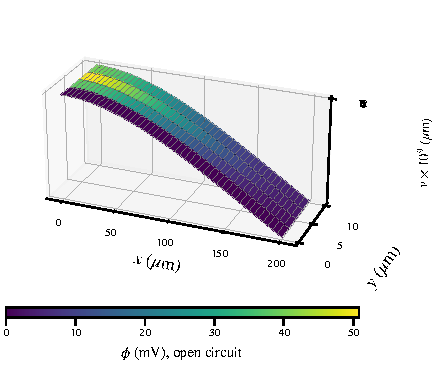
\includegraphics[width=0.62\textwidth]{P4_mode_shape_potential.pdf}
\caption{The extensional mode of the \SI{200}{\micro\metre}$\times$
\SI{10}{\micro\metre} plate, poling $x$, plotted as the deformed centre
surface with the small transverse displacement magnified by the factor printed
on the vertical axis (the true peak motion is \SI{10}{\nano\metre}) and the
open-circuit potential in colour.  The potential is the solution of the
electrode problem, not a post-hoc field: it is antisymmetric about the neutral
surface and reaches \SI{49}{mV} at the free end for
\SI{10}{nano\metre} of motion, which is the same number that the scalar
$d^{\rm T}\bm{\phi}/\beta$ gives.  Generated by
\texttt{python/run\_paper\_figures.py}.}
\label{fig:modeshape}
\end{figure}

\paragraph{Mode tracking, stated positively.}  Figure~\ref{fig:modetrack}
makes the same point from the other side: a single mode shape, identified once
at the thickest plate, is followed to $h=5,2,1$\,\si{\micro\metre} and compared
with it by modal assurance criterion, $\mathrm{MAC}=(\bm\phi_1^{\rm T}\bm
\phi_{\rm ref})^2/(\bm\phi_1^{\rm T}\bm\phi_1)(\bm\phi_{\rm ref}^{\rm T}\bm
\phi_{\rm ref})$.  The MAC stays above $0.9992$ down to \SI{1}{\micro\metre}
and every off-diagonal entry is below $2.3\times10^{-6}$ (checks K1, K2), so
the shape really is the same one at every thickness and the frequency ratio
$f_2/f_1$ stays above $6.2$: no mode crossing is involved.  That is the
numerical justification for the claim in Sec.~\ref{sec:orientation} that the
coupled mode is stable over a sweep -- the sweep changes the window, not the
mode, and this is what stability means when it is measured rather than
asserted.

\begin{figure}[t]
\centering
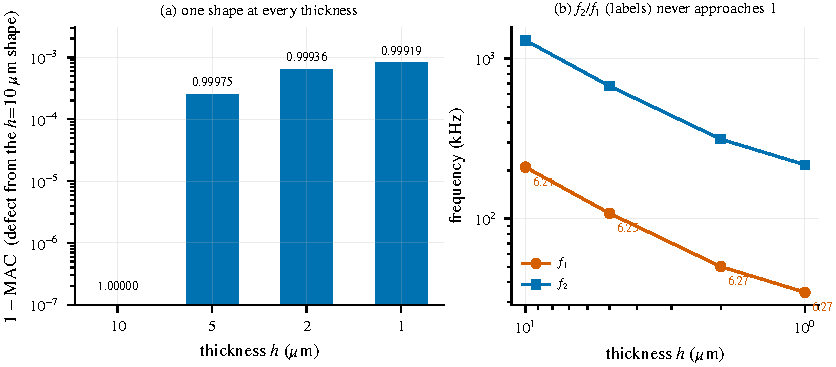
\includegraphics[width=0.78\textwidth]{P8_mode_tracking.pdf}
\caption{The same mode at four thicknesses.  (a) Defect $1-\mathrm{MAC}$
against the $h=\SI{10}{\micro\metre}$ shape, on a logarithmic axis: the worst
value is $8.1\times10^{-4}$.  The bar at $h=\SI{10}{\micro\metre}$ is the
reference itself and sits at the axis floor.  (b) The two lowest
short-circuit frequencies over the sweep, with $f_2/f_1$ printed at each
point: the ratio is $6.21$, $6.25$, $6.27$, $6.27$, so thinning the plate moves
both modes together and neither overtakes the other.  Numbers from
\texttt{results/mode\_tracking.json}.}
\label{fig:modetrack}
\end{figure}

\paragraph{A coupling map applied twice.}  The thickness sweep of
Fig.~\ref{fig:thickness}(b) first reported this plate's coupling as
$0.3582$, constant to $0.05\,\%$ over the range -- plausible, smooth, and
wrong.  The number came from a helper that evaluated \eqref{eq:kx} with the
\emph{open-circuit} matrix in place of $K_{uu}$:
$x'=d^{\mathsf T}K_{oc}^{-1}d/\beta$, and then applied $x/(1+x)$ to $x'$.
Because $K_{oc}$ is the rank-one update \eqref{eq:rankone},
\[
  \frac{d^{\mathsf T}K_{oc}^{-1}d}{\beta}
  =x-\frac{x^2}{1+x}=\frac{x}{1+x}=k^2
\]
by Sherman--Morrison, so the first substitution already returned $k^2$ and the
map turned it into $k^2/(1+k^2)$.  The identity reproduces the quoted series
digit for digit (Table~\ref{tab:wrongk}) -- which is what identifies the error
as an algebra slip rather than a different material, geometry or mesh, and is
why the closed form of Sec.~\ref{sec:closedform} is graded (check C1) rather
than trusted.  Two things made it visible: the closed form disagreed with the
finite element model by $56\,\%$, and the corrected value
$k^2=0.5581$ is the one the material constants predict.

\begin{table}[t]
\centering
\small
\caption{The superseded coupling series of Fig.~\ref{fig:thickness}(b), and
the corrected values it was produced from.  The fourth column is
$k^2/(1+k^2)$ evaluated on the third, to five decimals; it agrees with what the
earlier helper printed for all four thicknesses, which fixes the error as
\eqref{eq:kx} applied twice.  Generated by
\texttt{python/derive\_k2\_closed\_form.py}.}
\label{tab:wrongk}
% generated by python/derive_k2_closed_form.py -- do not edit
\begin{tabular}{@{}lccc@{}}
\toprule
$h$ (\si{\micro\metre}) & correct $k^2$ & $k^2/(1+k^2)$ & value that was quoted \\
\midrule
10 & 0.55814 & 0.35821 & 0.35821 \\
5 & 0.55843 & 0.35833 & 0.35833 \\
2 & 0.55858 & 0.35839 & 0.35839 \\
1 & 0.55861 & 0.35840 & 0.35840 \\
\bottomrule
\end{tabular}

\end{table}

\paragraph{Differencing two eigensolves.}  When $k^2\sim10^{-3}$, the two
eigenvalues of $(\omega_{oc}^2-\omega_{sc}^2)/\omega_{oc}^2$ agree to three
digits and the pencil has $\mathrm{cond}(K)\sim10^{12}$; the round-off of the
difference is the size of the answer.  With $\mu=0$, where the flexoelectric
coupling is identically zero by symmetry, the two-solve formula returned
$+7.5\times10^{-4}$ and $+4.4\times10^{-3}$ on two different meshes.  Because
$K_{oc}$ is a rank-one update of $K_{sc}$ (Eq.~\eqref{eq:rankone}), the
open-circuit fundamental frequency can instead be obtained as the root in
$(\omega_0^2,\omega_1^2)$ of
\begin{equation}
  1+\sum_i \frac{s_i}{\omega_i^2-y}=0,\qquad
  s_i=\frac{(d\cdot\bm{\phi}_i)^2}{\beta},
  \label{eq:secular}
\end{equation}
with $(\omega_i,\bm{\phi}_i)$ the mass-normalised \emph{short-circuit} modes.
One eigensolve, no difference of close eigenvalues (the eigenvector sign
cancels in $s_i$), and a strictly increasing function between poles, so
bisection is unconditionally safe.  The $\mu=0$ residual drops to
$1.0\times10^{-10}$, i.e.\ to round-off, and the result is mesh-stable
(check~T4).

%% ===========================================================================
\section{Results}
\label{sec:results}
%% ===========================================================================

\subsection{Window orientation and plate aspect ratio}
\label{sec:orientation}

Figures~\ref{fig:petals} and~\ref{fig:map} vary the orientation $\theta$ of the
rectangular averaging window and the plate aspect ratio, for the poling-$x$
(length-extensional) configuration that dominates the response.  The window is
held at a half-width of \SI{3}{\micro\metre} along its long axis; the plate is
\SI{200}{\micro\metre}$\times$\SI{10}{\micro\metre}; the extensional mode is
identified as the one carrying the largest coupling, an identification that is
stable over the sweep (its short-circuit frequency varies smoothly from
4907 to \SI{5296}{kHz} over all $6\times24$ cases).

Both quantities move monotonically with $\theta$ and both saturate by
$\theta=90^\circ$.  The extensional frequency rises from \SI{149.5}{kHz} to
\SI{158.3}{kHz} at ${\rm AR}=2$ and from \SI{146.4}{kHz} to \SI{158.1}{kHz}
at ${\rm AR}=10$ (6--8\,\%), while the axial-mode coupling falls from
$0.4448$ to $0.3786$ and from $0.4677$ to $0.3801$ over the same interval
(15--19\,\%).  At $\theta=0^\circ$ the window aspect ratio is worth
$0.4448\to0.4677$ between ${\rm AR}=2$ and ${\rm AR}=10$, i.e.\ about
5\,\%, and the aspect ratios collapse onto $0.3786$--$0.3801$ at
$\theta=90^\circ$: once the long axis of the window is transverse to the
strain gradient, its aspect ratio no longer matters.  The two figures show the
same data in the two geometries a reader may want: the polar plot reads the
angular dependence directly (the flower has its maxima at $\theta=0^\circ$ and
$180^\circ$ in $k^2$ and its minima there in $f_1$), the map reads the aspect
ratio.

Two remarks keep this in proportion.  First, the coupling plotted here is the
\emph{total} coupling of the extensional mode, and it is piezoelectric in the
main (the flexoelectric contribution at $\mu=10^{-6}$\,\si{\coulomb\per\metre}
is of order $10^{-4}$, Sec.~\ref{sec:thickness}); the window therefore acts on
the modal coupling through the gradient stiffness in $K_{sc}$, not by adding a
flexoelectric term directly.  Second, the same statement in the language of
Sec.~\ref{sec:window} is that rotating the window rotates $M$, and it is $M$
that the solution sees: the $15$--$19\,\%$ spread is a property of the
second-moment tensor of a rectangular window, not of the rectangle as such.

\begin{figure}[t]
\centering
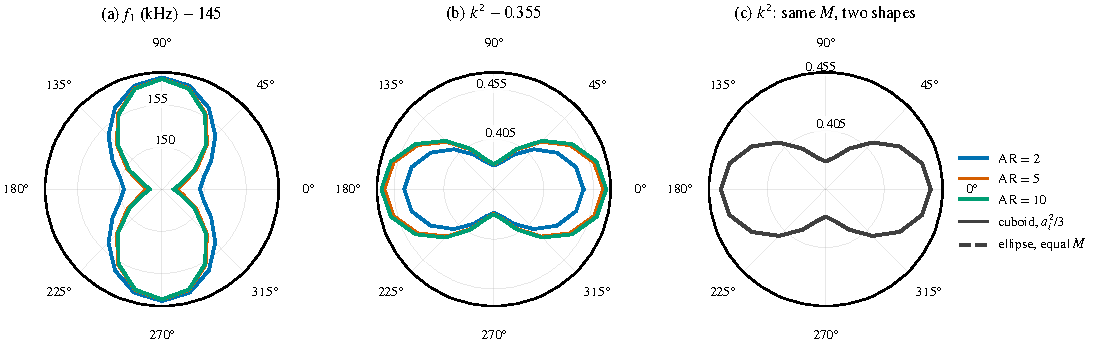
\includegraphics[width=\textwidth]{P2_petals.pdf}
\caption{Window orientation as a polar plot, drawn by
\texttt{python/run\_paper\_figures.py} from
\texttt{results/paper\_figures\_data.json}.  Radius is the quantity itself,
offset so that its variation is visible; the radial tick labels give the true
values.  (a) Fundamental frequency $f_1$ minus \SI{145}{kHz}; (b) coupling
$k^2$ of the extensional mode minus $0.355$; (c) the same $k^2$ for a cuboid
window of half-widths $3\times1.5$\,\si{\micro\metre} (solid) and an
elliptical window carrying the same second-moment tensor (dashed), which are
indistinguishable.  Plate \SI{200}{\micro\metre}$\times$\SI{10}{\micro\metre},
poling $x$, plane stress, $24\times2$ mesh, $\mu=0$.}
\label{fig:petals}
\end{figure}

\begin{figure}[t]
\centering
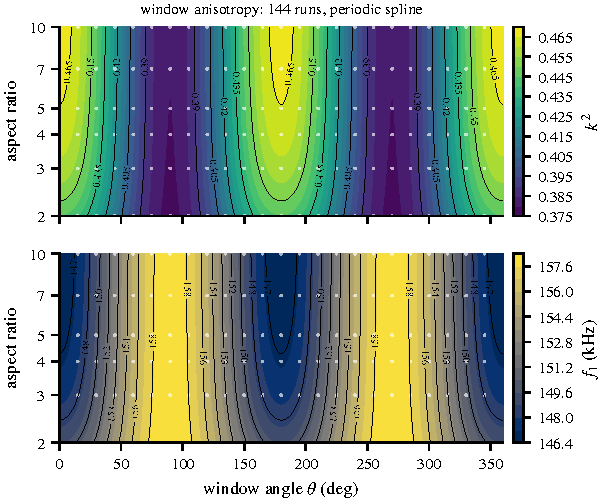
\includegraphics[width=0.62\textwidth]{P3_map_k2_AR_theta.pdf}
\caption{The same sweep as Fig.~\ref{fig:petals}, as a filled contour map over
the window angle and the aspect ratio: (top) extensional $k^2$, (bottom)
$f_1$.  Contours are a periodic spline through the $144$ computed points
(white dots); no data are extrapolated.  The coupling is maximal when the
long axis of the window is aligned with the strain ($\theta=0^\circ$,
$180^\circ$) and is flat in the aspect ratio at $\theta=90^\circ$, where the
window's anisotropy no longer enters the second-moment tensor.  Note the
anticorrelation of the two panels: the window orientation that maximises the
coupling is the one that minimises the frequency.}
\label{fig:map}
\end{figure}

\subsection{Fractional memory: which matrix is it, and against what?}
\label{sec:memorystudy}

Two questions are separated here.  The first is \emph{model}:
the fractional Kelvin--Voigt element of \eqref{eq:kv} is one way to represent
dielectric loss, and it is worth knowing how much it differs from the
alternative that is usually available in finite element codes, namely a
standard (integer-order) Kelvin--Voigt or Zener element fitted at the device
frequency.  The second is \emph{implementation}: the convolution of
\eqref{eq:step} may multiply the fully condensed stiffness $K_{\rm eff}$ or
only the short-circuit matrix $K_{uu}$, and the two give different damping.

\paragraph{Memory matrix.}  Table~\ref{tab:S1} reports the ring-down of the
extensional mode (mode 4, \SI{6.727}{MHz}, $k^2_{\rm eff}=0.4650$ with the
fully uncoupled $K_{uu}$ denominator of \eqref{eq:kstatic}; the short-circuit
denominator used in Table~\ref{tab:kinematics} gives $0.4580$ for the same mode,
and the $1.5\,\%$ difference is the contribution of the internal potential dofs
that grounding the electrodes does not remove -- the denominator has to be
named, which is the point of Sec.~\ref{sec:couplingcare}) at
$\tau=\SI{7.0974}{\nano\second}$, i.e.\ $\omega\tau=0.3$, with an initial tip
displacement that produces \SI{139.07}{\volt} of open-circuit voltage at
$t=0$.  The damping ratio extracted from the logarithmic decrement,
\eqref{eq:zeta}, is $0.15023$ for $K_{\rm eff}$ at $\alpha=1$, against the
exact $\omega\tau/2=0.15000$: the implementation reproduces the classical
limit to $0.15\,\%$.  Replacing $K_{\rm eff}$ by $K_{uu}$ removes the
piezoelectric contribution from the memory and takes the ratio
$\zeta(K_{uu})/\zeta(K_{\rm eff})$ at $\alpha=1$ down to $0.449$, i.e.\ the
short-circuit memory dissipates $55\,\%$ less.  The difference is of the order
of the coupling ($k^2_{\rm eff}=0.4650$) but does \emph{not} reduce to the
naive factor $1-k^2=0.535$: the two memories differ by the piezoelectric
stiffness that the condensation puts into $K_{\rm eff}$, and its effect on the
ring-down has to be computed rather than estimated.  For a strongly
piezoelectric device the distinction therefore belongs in the model statement,
not in the implementation.

\begin{table}[t]
\centering
\small
\caption{Ring-down of the extensional mode (mode 4, \SI{6.727}{MHz},
$k^2_{\rm eff}=0.4650$, $\omega\tau=0.3$, $\tau=\SI{7.0974}{\nano\second}$).
Damping ratio from the logarithmic decrement of \eqref{eq:zeta}.}
\label{tab:S1}
\begin{tabular}{@{}lcc@{}}
\toprule
memory matrix & $\alpha=1$ & $\alpha=0.7$ \\
\midrule
$K_{\rm eff}$ & $0.15023$ & $0.02600$ \\
$K_{uu}$      & $0.06749$ & $0.05006$ \\
\midrule
ratio $K_{uu}/K_{\rm eff}$ & $0.449$ & $1.93$ \\
\bottomrule
\end{tabular}
\end{table}

\paragraph{Against Kelvin--Voigt and Zener.}  Table~\ref{tab:S2} compares the
complex modulus of the fractional element, \eqref{eq:kvfreq}, with the
integer-order Kelvin--Voigt and Zener fits at the same relaxation time.  At
the device point $\omega\tau=0.3$ the Kelvin--Voigt model over-predicts the
modulus by $3.5\,\%$ at $\alpha=1$ and by $22.6\,\%$ at $\alpha=0.7$;
at $\omega\tau=1$ the ratio of the two is $1.345$ and $1.623$, and at
$\omega\tau=100$ the integer-order model is wrong by a factor $90.9$.  The
fractional model is not a cosmetic refinement: a single-relaxation fit is
unusable outside the narrow band where it was fitted, which is precisely the
band a design map is supposed to cover.

\begin{table}[t]
\centering
\small
\caption{Normalised modulus magnitude $|K^*|/K$ at matched $\tau$: the
integer-order Kelvin--Voigt element and the fractional Zener element with
relaxation-strength ratio $r=2$.  The ratio of the two is discussed in the
text.}
\label{tab:S2}
\begin{tabular}{@{}lcccc@{}}
\toprule
$\omega\tau$ & \multicolumn{2}{c}{$\alpha=1$} & \multicolumn{2}{c}{$\alpha=0.7$} \\
\cmidrule(lr){2-3}\cmidrule(lr){4-5}
 & KV & Zener ($r=2$) & KV & Zener ($r=2$) \\
\midrule
0.3  & $1.0440$ & $1.1170$ & $1.2555$ & $1.2652$ \\
1    & $1.4142$ & $1.5811$ & $1.7053$ & $1.5310$ \\
10   & $10.050$ & $1.9926$ & $5.5380$ & $1.8988$ \\
100  & $100.005$ & $1.9999$ & $25.588$ & $1.9814$ \\
\bottomrule
\end{tabular}
\end{table}

\subsection{The damping map}
\label{sec:damping}

Two representations of the same model are useful.  Figure~\ref{fig:locus} is
the pole of \eqref{eq:kvfreq} in the complex plane, traced over $\omega\tau$ for
seven relaxation times and coloured by the Caputo order; Fig.~\ref{fig:zetasurf}
is the damping ratio $\zeta=-\mathrm{Re}\,s/(\omega_0|s|)$ over the
$(\alpha,\omega\tau)$ plane.  Both are computed with branch continuation: the
root is followed from one $\omega\tau$ to the next by warm-starting the
Newton iteration at the previous pole.  Without that continuation the
iteration jumps to a spurious root of the negative-real-part branch, and the
map acquires a singularity that is an artefact of the solver, not of the
model -- it appeared in an earlier version of both panels and is the reason
they are described here.

The locus makes three points that a table cannot.  All poles lie in the left
half-plane for every $(\alpha,\tau)$ examined, so the fractional Kelvin--Voigt
element is dissipative by construction.  The integer-order case
($\alpha=1$, open markers) sits at $|\mathrm{Im}\,s|/\omega_0\simeq1$ for
$\omega\tau\lesssim0.1$ and moves down and right as $\omega\tau$ grows: the
dashpot lowers the frequency and eventually over-damps the mode.  The
fractional cases ($\alpha<1$) start from the same neighbourhood and fan
\emph{upward}: a spring-pot with $\alpha<1$ raises the damped frequency as
$\tau$ grows, because the fractional modulus grows sub-linearly rather than
linearly in $\omega$.  The order of magnitude of the effect is the point: at
$\alpha=0.5$ and $\omega\tau=10$ the damped frequency is $2.13\,\omega_0$
($2.45\,\omega_0$ at $\alpha=0.7$), against $\mathrm{Im}\,s=0$ -- complete
over-damping -- for $\alpha=1$ at the same $\omega\tau$.  A single-fit
Kelvin--Voigt parameterisation cannot reproduce that; the pole, not the
modulus, is what a design should be read from.

Figure~\ref{fig:zetasurf} reads the same information as a design surface:
$\zeta$ increases with both $\alpha$ and $\omega\tau$ and saturates at
$\zeta=1$ for $\alpha\to1$ and large $\omega\tau$, where the element is
critically damped.  For small $\alpha$ the surface is flat: a
spring-pot with a broad relaxation spectrum produces a damping that depends
only weakly on the device frequency, which is the qualitative reason the
fractional description is used for dielectric loss in the first place.
Together with Table~\ref{tab:S1} this gives the design map: for a given device
frequency the pair $(\alpha,\tau)$ fixes the damping, and the map must be read
with the memory matrix that the model actually uses.

\begin{figure}[t]
\centering
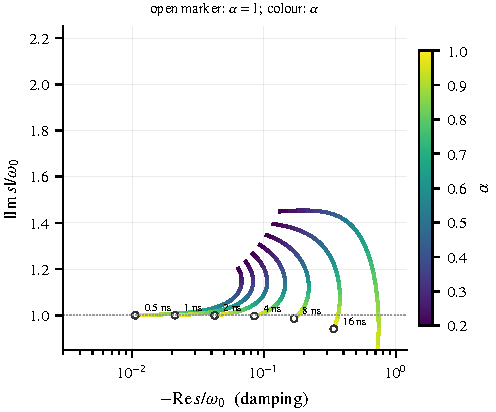
\includegraphics[width=0.52\textwidth]{P5_root_locus.pdf}
\caption{Complex poles of the fractional Kelvin--Voigt element,
$s/\omega_0$ in the plane $(-\mathrm{Re},\mathrm{Im})$, traced over
$\omega\tau=0.01\ldots31.6$ for seven relaxation times (labels, at the last
point of each curve), coloured by the Caputo order.  Open markers are
$\alpha=1$.  The dotted line is $\mathrm{Im}\,s=\omega_0$.  Every pole has a
negative real part; the fractional curves fan upward because the spring-pot
modulus grows sub-linearly in frequency.  Generated by
\texttt{python/run\_paper\_figures.py}.}
\label{fig:locus}
\end{figure}

\begin{figure}[t]
\centering
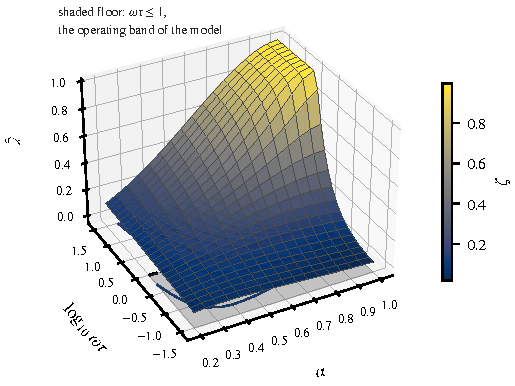
\includegraphics[width=0.55\textwidth]{P9_damping_surface.pdf}
\caption{Damping ratio of the same element over the
$(\alpha,\omega\tau)$ plane, from the complex pole with branch continuation.
The surface is drawn only where three variables are present; the projection at
the base repeats the same data as contours.  Saturation at $\zeta=1$ for
$\alpha\to1$ is critical damping of the integer-order dashpot.}
\label{fig:zetasurf}
\end{figure}

\subsection{Window shape versus second moment}
\label{sec:windowresult}

Figure~\ref{fig:domain} is the numerical statement of Sec.~\ref{sec:window} on
an isotropic plane-strain test problem (rectangle $1\times0.2$, $20\times4$
mesh, uniaxial edge traction, displacement $u_R$ averaged over the loaded
edge).  The response is plotted against the normalized window size for an
ellipsoidal window of semi-axis $l$, a cuboidal window of half-width $l$, and
a cuboidal window scaled to have the same $M$ as the ellipsoid,
$a=l\sqrt{3/5}$.  The third curve is indistinguishable from the first: the
window's shape is irrelevant at fixed $M$, and only $M$ enters the model.  The
second curve shows the error that is made by ignoring the distinction: taking
equal half-widths instead of equal $M$ over-stiffens the response, and the
discrepancy grows with the window size.  At $l/L_x=0.2$ a cuboid of
half-width $l$ retains $0.921$ of the classical loaded-edge displacement, an
ellipsoid of semi-axis $l$ retains $0.941$, and the equal-$M$ cuboid sits on
the ellipsoid curve to the third decimal: at fixed $M$ the shape of the window
is immaterial to $10^{-3}$, which is the coefficient ratio $5/3$ in $K_g$ of
check V1d seen from the response side.

\begin{figure}[t]
\centering
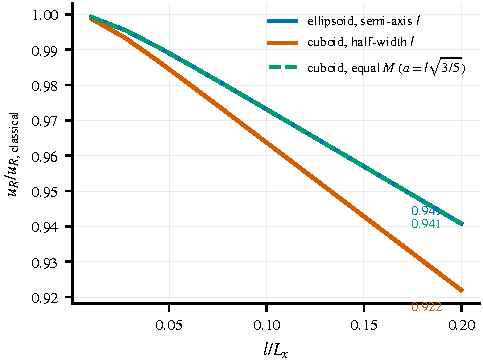
\includegraphics[width=0.55\textwidth]{P10_window_shape.pdf}
\caption{Loaded-edge displacement versus window size for an ellipsoidal window
(semi-axis $l$), a cuboidal window (half-width $l$), and a cuboidal window
scaled to the same second moment, $a=l\sqrt{3/5}$.  Isotropic plane-strain
test problem (rectangle $1\times0.2$, $20\times4$ mesh, uniaxial edge
traction), response normalized by its classical value with no gradient term.
The two curves that share $M$ coincide; the curve that shares a half-width
does not.  Numbers at $l/L_x=0.2$ are printed on the curves.}
\label{fig:domain}
\end{figure}

\subsection{Thickness: a flexoelectric size effect against a
thickness-independent piezoelectric coupling}
\label{sec:thickness}

Figure~\ref{fig:thickness} is the central design result.  The same plate is
solved at $h=10,5,2,1$\,\si{\micro\metre} with a \SI{200}{\micro\metre} length,
and the window held fixed at half-widths $3\times1$\,\si{\micro\metre}, so
that the thickness is the only variable.  The two panels are two electrical
configurations of that plate, not two estimates of one number: panel~(a) is
poled across the thickness (electrodes on the long faces, gap $h$,
$\kappa_{yy}=\kappa_{33}$) and panel~(b) along the length (electrodes on the
short faces, gap $L$, $\kappa_{xx}=\kappa_{33}$), as set out in
Table~\ref{tab:axes}.  Panel~(a) is the flexoelectric
bending coupling with $\mu=10^{-6}$\,\si{\coulomb\per\metre} (a \emph{nominal}
value: no measured flexoelectric coefficient for BaTiO$_3$ is used here, and
the whole panel scales as $\mu^2$); panel~(b) is the piezoelectric
length-extensional coupling of the same plate, evaluated with $\mu=0$ and with
the mode-free measure \eqref{eq:kstatic}.

\paragraph{Flexoelectric size effect.}  The flexoelectric coupling rises by a
factor $23.9$ from \num{1.74e-4} at \SI{10}{\micro\metre} to
\num{4.17e-3} at \SI{1}{\micro\metre}.  The local log-log slope is $-1.92$ at
the thick end, i.e.\ the expected $h^{-2}$ scaling, and steepens to $-1.52$ and
then $-0.66$ as the plate is thinned.  The saturation is not a mesh artefact:
the $96\times4$ witness reproduces the $48\times4$ values to $0.04\,\%$ and
$0.35\,\%$ at the two ends of the range (check T4), and the residual at
$\mu=0$ is $1.0\times10^{-10}$ (check T5), seven orders of magnitude below the
signal.  Its physical reading -- that the fixed
\SIrange{3}{1}{\micro\metre} averaging window becomes comparable to the
thickness and smears the through-thickness strain gradient -- is an
interpretation, not a measurement of this study; the same stiffening appears
in the fundamental frequency, which follows
$210.4, 108.0, 50.2, 34.7$\,kHz where pure Euler--Bernoulli scaling from the
thickest plate would give $210, 105, 42, 21$\,kHz.

\paragraph{Piezoelectric coupling is thickness independent.}  Panel~(b) gives
$k^2 = 0.55814, 0.55843, 0.55858, 0.55861$ for the four thicknesses: a
variation of $0.09\,\%$ (check T1), mesh independent to $5.7\times10^{-4}$
(check T2), against the mode-free closed-form value $0.56079$ for the same
material and the same plane-stress kinematics (check C1).  This is the statement that makes the pair useful.  The
piezoelectric effect is a \emph{bulk} effect and a thinner plate is
electromechanically neither better nor worse; the flexoelectric effect is a
gradient effect and improves by more than an order of magnitude over the same
range.  A device can therefore be thinned for the flexoelectric response
without a penalty in the piezoelectric one, and the crossover thickness is a
property of the window and of $\mu$, not of the piezoelectric constants.

\begin{figure}[t]
\centering
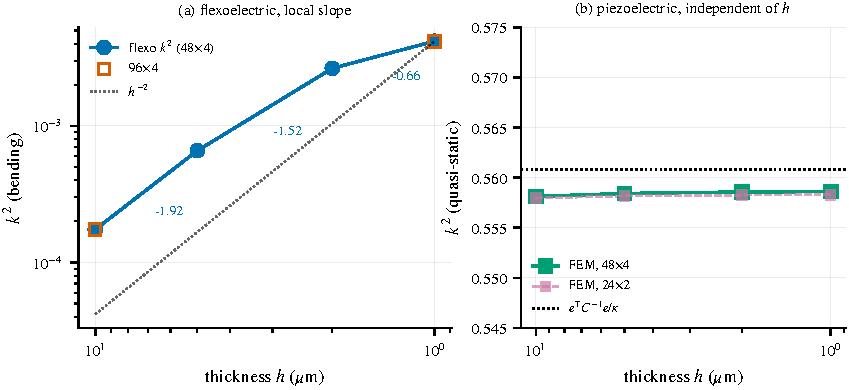
\includegraphics[width=\textwidth]{P7_thickness.pdf}
\caption{(a) Flexoelectric bending coupling versus plate thickness
($L=\SI{200}{\micro\metre}$, window half-widths
$3\times1$\,\si{\micro\metre}, $\mu=10^{-6}$\,\si{\coulomb\per\metre}), with
the local log--log slopes annotated, a $96\times4$ witness at the two thickest
and thinnest points (open squares, indistinguishable from $48\times4$), and
the $h^{-2}$ guide line.  (b) Piezoelectric length-extensional coupling of the
same plate with $\mu=0$, mode-free: constant to $0.09\,\%$ over
$10\to1$\,\si{\micro\metre}, and $0.4\,\%$ below the closed form
$e^{\rm T}C^{-1}e/\kappa=0.56079$ (dotted), which is the discretisation error
of the $48\times4$ mesh, not a modelling difference.  Numbers from
\texttt{results/demo.json}.}
\label{fig:thickness}
\end{figure}

\subsection{Transient response and the memory model}
\label{sec:transient}

Figure~\ref{fig:ringdown} shows the ring-down of the extensional mode after an
initial displacement of \SI{10}{\nano\metre} at the tip, for four Caputo
orders and fixed $\tau=\SI{3}{\nano\second}$: the tip displacement in
panel~(a) and the open-circuit voltage in panel~(b).  The initial voltage,
\SI{139}{\volt}, is set by the mode shape and the electrode configuration and
is independent of $\alpha$ -- as it must be, since the memory term vanishes at
$t=0^+$ -- while the decay rate depends strongly on $\alpha$.  The $\alpha=1$
curve is the exponential decay of the classical Kelvin--Voigt element; the
fractional curves are not exponential, and it is that difference which the
damping map of Figs.~\ref{fig:locus} and~\ref{fig:zetasurf} quantifies.  The
voltage is a linear functional of the same modal coordinate, so it inherits
the ring-down shape; what the figure is meant to make visible is that a design
calibrated on the integer-order decay is optimistic or pessimistic by a factor
of order two, depending on the sign of the difference between $\alpha$ and the
order that fits the measured loss.

\begin{figure}[t]
\centering
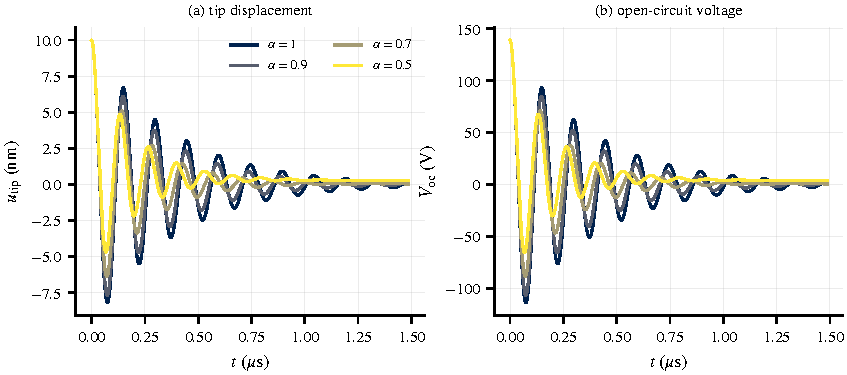
\includegraphics[width=\textwidth]{P6_ringdown.pdf}
\caption{Ring-down of the extensional mode of the
\SI{200}{\micro\metre}$\times$\SI{10}{\micro\metre} plate at its first
strongly coupled mode for $\alpha=1,0.9,0.7,0.5$: (a) tip displacement,
(b) open-circuit voltage.  Modal memory on $K_{\rm eff}$, eight modes,
$\tau=\SI{3}{\nano\second}$, initial tip displacement \SI{10}{\nano\metre}.
Each curve is an independent L1 time march; the four share the initial
condition and differ only in $\alpha$.  Generated by
\texttt{python/run\_paper\_figures.py}.}
\label{fig:ringdown}
\end{figure}

%% ===========================================================================
\section{Application: a \SI{200}{\micro\metre} by \SI{10}{\micro\metre} energy harvester}
\label{sec:application}
%% ===========================================================================

The worked case throughout is a \SI{200}{\micro\metre} long,
\SI{10}{\micro\metre} thick BaTiO$_3$ plate, clamped on one short edge, poled
along its length and electroded on the two ends.  In this configuration the
strain in the active region is extensional rather than bending, so the
piezoelectric coupling is the larger of the two and the flexoelectric term is
a size-dependent correction rather than the main effect.  Table~\ref{tab:kinematics}
collects the numbers from the run; they are the numbers a designer needs
before choosing between the extensional and the bending configuration.

Table~\ref{tab:kinematics} is the whole of it: the same plate in the four
polarisation/kinematics combinations, each with the frequency of the mode that
carries its coupling.

Three consequences follow from the runs and are worth stating explicitly.

\begin{enumerate}
\item \textbf{Polarisation direction dominates everything else.}  The
  length-extensional configuration with poling along the length gives
  $k^2=0.4580$ and \SI{138.99}{\volt} at the same \SI{10}{\nano\metre} of
  motion; the bending configuration gives $0.1141$ and \SI{2.41}{\volt}, a
  factor $58$ in voltage at equal amplitude and a factor four in $k^2$.  A
  device that excites bending and hopes to harvest through $e_{31}$ is working
  against that handicap at this geometry -- and the handicap is not a
  property of $e_{31}$ but of the electrode arrangement that bending
  requires, since a symmetric plate bent between full through-thickness
  electrodes produces almost no net charge: the fundamental bending mode has
  $k^2=2.3\times10^{-10}$ (check V4a), the mode that couples through the
  thickness being the fourth.
\item \textbf{The quasi-static coupling of the same plate is $0.5581$} and is
  thickness independent (Sec.~\ref{sec:thickness}).  This is the number to
  quote for a device whose operating frequency is far below its first
  resonance, and it is the number that remains meaningful when the plate is
  thinned for the flexoelectric contribution.
\item \textbf{The damping is set by $(\alpha,\tau)$ and by the memory matrix},
  not by a material constant.  For the extensional mode of this plate at
  $\omega\tau=0.3$, $\zeta_{\rm eff}$ runs from $0.150$ ($K_{\rm eff}$,
  $\alpha=1$) to $0.026$ ($K_{\rm eff}$, $\alpha=0.7$) and to $0.067$
  ($K_{uu}$, $\alpha=1$).  Any design that reports a single damping number
  without naming $\alpha$, $\tau$ and the memory matrix is under-specified.
\end{enumerate}

%% ===========================================================================
\section{Limitations and unverified items}
\label{sec:limitations}
%% ===========================================================================

The following are stated here rather than buried, because each one bounds a
claim made above.

\begin{enumerate}
\item \textbf{Density.} $\rho=\SI{6020}{\kilo\gram\per\cubic\metre}$ is not
  verified against a primary source in this work.  Every frequency scales as
  $\rho^{-1/2}$; the coupling factors, the size-effect ratio and the damping
  ratios do not depend on it.  It must be sourced before the frequencies are
  quoted as predictions.
\item \textbf{Flexoelectric coefficient.} $\mu$ is unmeasured for the material
  used here.  Panel~(a) of Fig.~\ref{fig:thickness} is a parametric study: the
  coupling scales as $\mu^2$ and the constant-strain patch test
  (check~F2) fixes only the \emph{implementation}, not the material.  The
  $1.25\times10^{-4}$ bending coupling of check~F4 at
  $\mu=10^{-6}$\,\si{\coulomb\per\metre} is therefore a sensitivity, not a
  prediction for BaTiO$_3$.
\item \textbf{Plane stress.}  The 2-D reduction is a modelling choice, not a
  consequence of the formulation, and Table~\ref{tab:kinematics} shows it is
  worth $12\,\%$ in $k^2$ for the extensional case and $35\,\%$ for the
  $y$-coupled one; the 2-D plane-stress value itself sits $2.8\,\%$ below the
  three-dimensional free-bar closed form (check C2, Sec.~\ref{sec:couplingcare}),
  which is the part of the gap that no choice of kinematics removes.  A three-dimensional
  implementation would remove the choice; this one does not.
\item \textbf{Interpretation of the saturation.}  The flattening of the
  flexoelectric curve below $h\approx\SI{2}{\micro\metre}$ is converged but
  its attribution to the window-to-thickness ratio is not separated in this
  study from the gradient-elastic stiffening of the thin plate, which is
  visible in the same runs through $f_1$.
\item \textbf{Fractional order.}  $\alpha$ and $\tau$ are treated as
  parameters.  Nothing here extracts them from a measurement, and the L1
  scheme used is first order in time; the reported orders ($0.99$ at
  $\alpha=1$) confirm that it is delivered as intended, not that it is the
  most efficient available.
\item \textbf{Two dimensions.}  The framework is plane; the $C^1$ BFS element
  is a rectangle, so curved and skewed geometries require either a
  mapped element or a different $C^1$ family.
\end{enumerate}

%% ===========================================================================
\section{Conclusions}
\label{sec:conclusions}
%% ===========================================================================

A $C^1$ Bogner--Fox--Schmit framework has been developed for
piezoelectric--flexoelectric strain-gradient plates with fractional-order
dielectric memory and a rectangular nonlocal averaging window, and verified
against a single-command suite of fifty-one checks in which every failure
mode that was found during the work is now a graded criterion.

The three contributions are the ones stated in the introduction.  Fractional
memory is carried on the modal coordinates with the L1 scheme, and the
distinction between the two candidate memory matrices is quantified rather
than assumed: the damping ratio for memory on the short-circuit matrix is
$0.449$ times that for memory on the fully condensed one at $\alpha=1$, a
$55\,\%$ reduction in dissipation that does not reduce to the naive $1-k^2$
factor for a device with $k^2=0.4650$ (uncoupled denominator; $0.4580$ on
the short-circuit one).  The
rectangular window enters only through its second-moment tensor $M$, with the
closed forms $a^2/3$, $a^2/4$ and $a^2/5$ for the cuboid, ellipse and
ellipsoid; two windows with equal $M$ produce identical results, and the
coefficient ratio at equal half-width is exactly $5/3$.  The open/short-circuit
coupling factor and the damping ratio together give a design map, and its
central entry is the contrast in Fig.~\ref{fig:thickness}: over
$10\to1$\,\si{\micro\metre} the flexoelectric bending coupling rises by a
factor $23.9$ while the piezoelectric extensional coupling of the same plate
is constant to $0.09\,\%$.

The methodological lesson is worth as much as the numbers.  Two of the
quantities reported here are differences of nearly equal eigenvalues, and both
produced smooth, plausible, wrong trends before they were reformulated -- a
mode-selection artefact that marched through the mode index as the plate was
thinned, and a two-eigensolve difference whose round-off equalled the answer.
The replacements (a mode-free static coupling and the secular equation of the
rank-one open-circuit update) are cheap, and they are what makes the numbers in
this paper reproducible by anyone who runs the same command.

\section*{Acknowledgment}

Financial support from the Haryana State Research Fund (HSRF), Government of
Haryana, under sanction number 14/66-2026 SPD/HSHEC/HSRF, is gratefully
acknowledged.

%% ===========================================================================
\bibliographystyle{elsarticle-num}
\begin{thebibliography}{99}

\bibitem{fem1}
%% TODO self-citation: restore the full reference from the delivered FEM-1
%% package (title, journal, volume, pages, year, DOI).
Authors of the FEM-1 paper,
\emph{$C^1$ plate finite element for piezoelectric strain-gradient
laminates}, reference to be completed from the FEM-1 delivery.

\bibitem{fem4}
%% TODO self-citation: full reference from the delivered FEM-4 package.
Authors of the FEM-4 paper,
\emph{Coupled piezoelectric--flexoelectric Mindlin Form-II continua},
reference to be completed from the FEM-4 delivery.

\bibitem{fem5}
%% TODO self-citation: full reference from the delivered FEM-5 package.
Authors of the FEM-5 paper,
\emph{Plate and shell implementation of the coupled piezoelectric--flexoelectric
model}, reference to be completed from the FEM-5 delivery.

\bibitem{mindlin}
R.~D. Mindlin,
Micro-structure in linear elasticity,
\emph{Archive for Rational Mechanics and Analysis} 16 (1964) 51--78.

\bibitem{toupin}
R.~A. Toupin,
Elastic materials with couple-stresses,
\emph{Archive for Rational Mechanics and Analysis} 11 (1962) 385--414.

\bibitem{bfs}
F.~K. Bogner, R.~L. Fox, L.~A. Schmit,
The generation of inter-element-compatible stiffness and mass matrices by the
use of interpolation formulas,
in: \emph{Proceedings of the Conference on Matrix Methods in Structural
Mechanics}, Wright--Patterson Air Force Base, 1965 (published 1966), pp.\
397--443.

\bibitem{zgonik}
M.~Zgonik, P.~Bernasconi, M.~Duelli, R.~Schlesser, P.~G\"unter,
Dielectric, elastic, piezoelectric, electro-optic, and elasto-optic tensors of
BaTiO$_3$ crystals,
\emph{Physical Review B} 50 (1994) 5941--5949.

\bibitem{caputo}
M.~Caputo,
Linear models of dissipation whose $Q$ is almost frequency independent---II,
\emph{Geophysical Journal of the Royal Astronomical Society} 13 (1967)
529--539.

\bibitem{bagley}
R.~L. Bagley, P.~J. Torvik,
A theoretical basis for the application of fractional calculus to
viscoelasticity,
\emph{Journal of Rheology} 27 (1983) 201--210.

\bibitem{koeller}
R.~C. Koeller,
Applications of fractional calculus to the theory of viscoelasticity,
\emph{Journal of Applied Mechanics} 51 (1984) 299--307.

\end{thebibliography}

\end{document}
